% !Mode:: "TeX:UTF-8"
\chapter{First Glance of Visual SLAM}
\begin{mdframed}
	\textbf{Goal of Study}
	\begin{enumerate}[labelindent=0em,leftmargin=1.5em]
		\item Understand which modules a visual SLAM framework consists of, and what task each module carries out.
		\item Set up the programming environment, and prepare for experiments.
		\item Understand how to compile and run a program under Linux. If there is a problem, how to debug it.
		\item Learn the basic usage of cmake.
	\end{enumerate}
\end{mdframed}

\newpage
\section{Introduction}

This lecture summarizes the structure of a visual SLAM system as an outline of subsequent chapters. Practice part introduces the fundamentals of environment setup and program development. We will make a small ``Hello SLAM'' program at the end.

\section{Meet ``Little Carrot''}

Suppose we assembled a robot called \emph{Little Carrot}, as shown in the following figure:

\begin{figure}
	\centering
	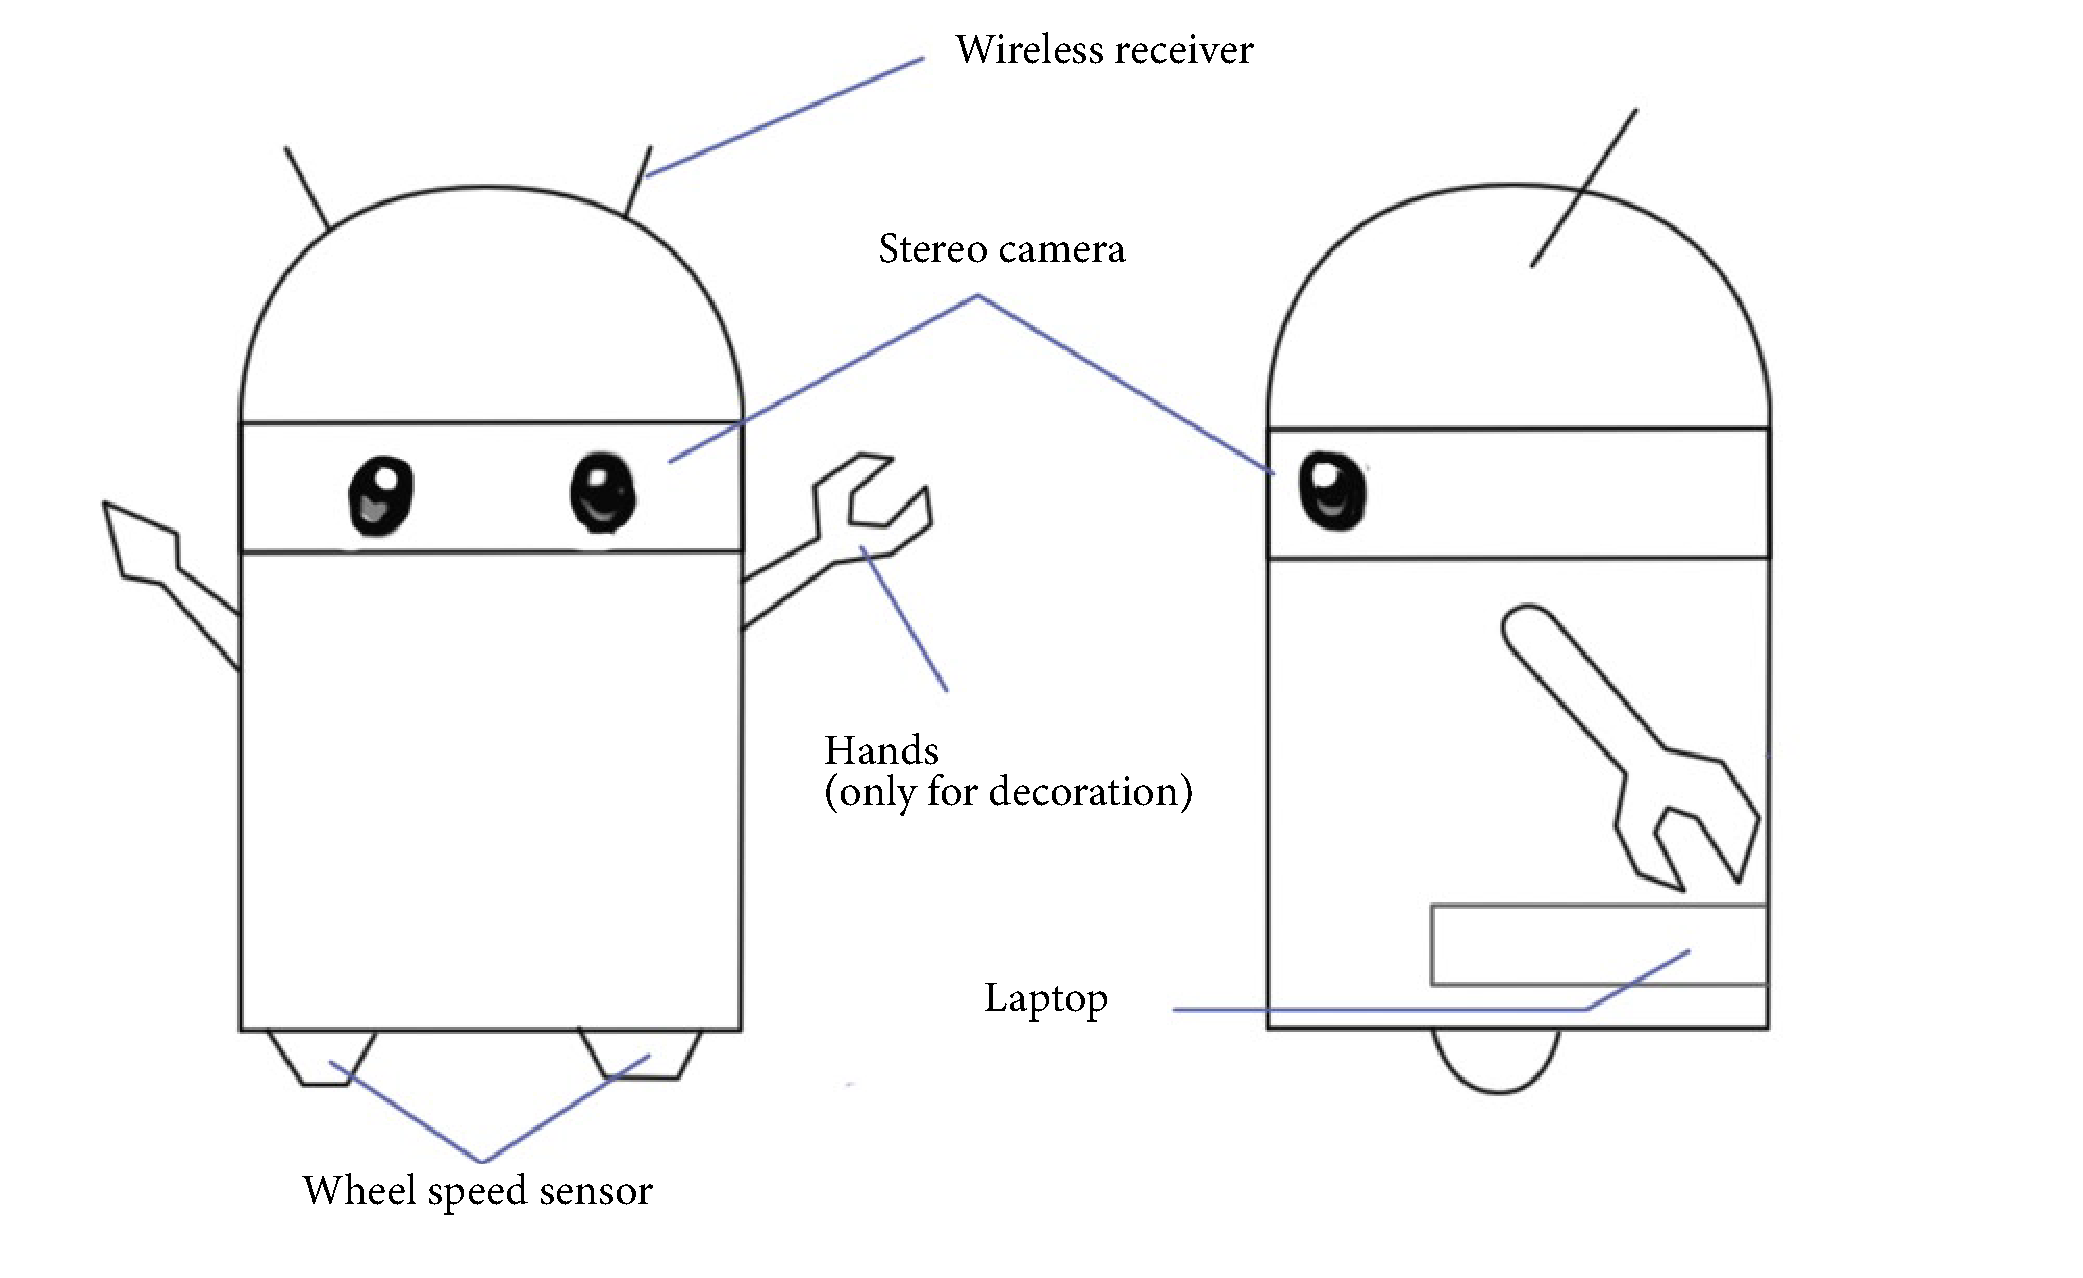
\includegraphics[width=0.8\textwidth]{resources/whatIsSLAM/carrot.pdf}
	\caption{The sketch of robot \emph{Little Carrot}}
\end{figure}

Although it looks a bit like the Android robot, it has nothing to do with the Android system. We put a laptop into its trunk (so that we can debug programs at any time). So, what is our robot capable to do?

We hope Little Carrot has the ability of \emph{autonomous moving}. Although there are many \emph{robots} placed statically on desktops, capable of chatting with people or playing music, but a tablet computer nowadays can also deliver the same tasks. As a robot, we hope Little Carrot can move freely in a room. Wherever we say hello to it, it can come to us right away.

First of all, such a robot needs wheels and motors to move, so we installed wheels under Little Carrot (gait control for humanoid robots is very complicated, which we will not be considering here). Now with the wheels, the robot is able to move, but without an effective navigation system, Little Carrot does not know where a target of action is, and it can do nothing but wander around blindly. Even worse, it may hit a wall and cause damage. In order to avoid this, we installed cameras on its head, with the intuition that such a robot \emph{should look similar to human}. Certainly, with eyes, brains and limbs, human can walk freely and explore any environment, so we (somehow naively) think that our robot should be able to achieve it too. Well, in order to make Little Carrot able to explore a room, we find it at least needs to know two things:

\begin{enumerate}
	\item  Where am I? - It's about \emph{localization}.
	\item What is the surrounding environment like? -It's about \emph{map building}.
\end{enumerate}

\emph{Localization} and \emph{map building}, can be seen as the perception in both inward and outward directions. As a completely autonomous robot, Little Carrot need not only to understand its own \emph{state} (i.e.\ the location), but also the external \emph{environment} (i.e.\ the map). Of course, there are many different approaches to solve these two problems. For example, we can lay guiding rails on the floor of the room, or paste a lot of artificial markers such as QR code pictures on the wall, or mount radio positioning devices on the table. If you are outdoor, you can also install a GNSS receiver (like the one in a cell phone or a car) on the head of Little Carrot. With these devices, can we claim that the positioning problem has been resolved? Let's categorize these sensors (see Fig.~\ref{fig:sensors}) into two classes.

\begin{figure}
	\centering
	\includegraphics[width=0.8\textwidth]{./resources/whatIsSLAM/sensors.jpg}
	\caption{Different kinds of sensors: (a) QR code (b) GNSS receiver (c) guiding rails (d) Laser range finder (e) Inertial measurement unit (f) stereo camera }
	\label{fig:sensors}
\end{figure}

The first class are \emph{non-intrusive} sensors which are completely self-contained inside a robot, such as wheel encoders, cameras, laser scanners, etc. They do not assume an cooperative environment around the robot. The other class are \emph{intrusive} sensors depending on a prepared environment, such as the above mentioned guiding rails, QR codes, etc. Intrusive sensors can usually locate a robot directly, solving the positioning problem in a simple and effective manner. However, since they require changes on the environment, the scope of usage is often limited within a certain degree. For example, if there is no GPS signal, or guiding rails cannot be laid, what should we do in those cases?

We can see that the intrusive sensors place certain \emph{constraints} to the external environment. A localization system based on them can only function properly when those constraints are met in the real world. Otherwise, the localization approach cannot be carried out anymore, like GPS positioning system normally doesn't work well in indoor environments. Therefore, although this type of sensor is simple and reliable, they do not work as a general solution. In contrast, non-intrusive sensors, such as laser scanners, cameras, wheel encoders, Inertial Measurement Units (IMUs), etc., can only observe indirect physical quantities rather than the direct locations. For example, a wheel encoder measures the wheel rotation angle, an IMU measures the angular velocity and the acceleration, a camera or a laser scanner observe the external environment in a certain form like point-clouds and images. We have to apply algorithms to infer positions from these indirect observations. While this sounds like a roundabout tactic, the more obvious benefit is that it does not make any demands on the environment, making it possible for this localization framework to be applied to an unknown environment. Therefore, they are called as self-localization in many research area.

Looking back at the SLAM definitions discussed earlier, we emphasized an \emph{unknown environment} in SLAM problems. In theory, we should not presume which environment the Little Carrot will be used (but in reality we will have a rough range, such as indoor or outdoor), which means that we can not assume that the external sensors like GPS can work smoothly. Therefore, the use of portable non-intrusive sensors to achieve SLAM is our main focus. In particular, when talking about visual SLAM, we generally refer to the using of \emph{cameras} to solve the localization and map building problems.

Visual SLAM is the main subject of this book, so we are particularly interested in what the Little Carrot's eyes can do. The cameras used in SLAM are different from the commonly seen Single Lens Reflex (SLR) cameras. It is often much simpler and does not carry expensive lens. It shoots at the surrounding environment at a certain rate, forming a continuous video stream. An ordinary camera can capture images at 30 frames per second, while high-speed cameras can do faster. The camera can be roughly divided into three categories: Monocular, Stereo and RGB-D, as shown by the following figure~\ref{fig:cameras}. Intuitively, a monocular camera has only one camera, a stereo camera has two. The principle of a RGB-D camera is more complex, in addition to being able to collect color images, it can also measure the distance of the scene from the camera for each pixel. RGB-D cameras usually carry multiple cameras, and may adopt a variety of different working principles. In the fifth lecture, we will detail their working principles, and readers just need an intuitive impression for now. In addition, there are also specialty and emerging camera types can be applied to SLAM, such as panorama camera~\cite{Pretto2011}, event camera~\cite{Rueckauer2016}. Although they are occasionally seen in SLAM applications, so far they have not become the mainstream. From the appearance we can infer that Little Carrot seems to carry a stereo camera.

\begin{figure}
	\centering
	\includegraphics[width=0.8\textwidth]{./resources/whatIsSLAM/camera.pdf}
	\caption{Different kinds of cameras: monocular, RGB-D and stereo. }
	\label{fig:cameras}
\end{figure}

Now, let's take a look at the pros and cons of using different type of camera for SLAM.

\subsubsection{Monocular Camera}

The SLAM system that uses only one camera is called Monocular SLAM. This sensor structure is particularly simple, and the cost is particularly low, therefore the monocular SLAM has been very attractive to researchers. You must have seen the output data of a monocular camera: photo. Yes, as a photo, what are its characteristics?

A photo is essentially a \emph{projection} of a scene onto a camera's imaging plane. It reflects a three-dimensional world in a two-dimensional form. Obviously, there is one dimension lost during this projection process, which is the so-called depth (or distance). In a monocular case, we can not obtain the \emph{distance} between objects in the scene and the camera by using a single image. Later we will see that this distance is actually critical for SLAM. Because we human have seen a large number of images, we formed a natural sense of distances for most scenes, and this can help us determine the distance relationship among the objects in the image. For example, we can recognize objects in the image and correlate them with their approximate size obtained from daily experience. The close objects will occlude the distant objects; the sun, the moon and other celestial objects are infinitely far away; an object will have shadow if it is under sunlight. This common sense can help us determine the distance of objects, but there are also certain cases that confuse us, and we can no longer determine the distance and true size of an object. The following figure~\ref{fig:why-depth} is shown as an example. In this image, we can not determine whether the figures are real person or small toys purely based on the image itself. Unless we change our view angle, explore the three-dimensional structure of the scene. In other words, from a single image, we can not determine the true size of an object. It may be a big but far away object, but it may also be a close but small object. They may appear to be the same size in an image due to the perspective projection effect.

\begin{figure}
	\centering
	\includegraphics[width=0.8\textwidth]{./resources/whatIsSLAM/why-depth.pdf}
	\caption{We cannot tell if the people are real humans or just small toys from a single image}
	\label{fig:why-depth}
\end{figure}

Since the image taken by an monocular camera is just a 2D projection of the 3D space, if we want to recover the 3D structure, we have to change the camera's view angle. Monocular SLAM adopts the same principle. We move the camera and estimate its own \emph{motion}, as well as the distances and sizes of the objects in the scene, namely the \emph{structure} of the scene. So how should we estimate these movements and structures? From the everyday experience we know that if a camera moves to the right, the objects in the image will move to the left which gives us an inspiration of inferring motion. On the other hand, we also know that closer objects move faster, while distant objects move slower. Thus, when the camera moves, the movement of these objects on the image forms pixel disparity. Through calculating the disparity, we can quantitatively determine which objects are far away and which objects are close.

However, even if we know which objects are near and which are far, they are still only relative values. For example, when we are watching a movie, we can tell which objects in the movie scene are bigger than the others, but we can not determine the \emph{real size} of those objects -- are the buildings real high-rise buildings or just models on a table? Is it a real monster that destructs a building, or just an actor wearing special clothing? Intuitively, if the camera's movement and the scene size are doubled at the same time, monocular cameras see the same. Likewise, multiplying this size by any factor, we will still get the same picture. This demonstrates that the trajectory and map obtained from monocular SLAM estimation will differ from the actual trajectory and map with a factor, which is just the so-called \emph{scale} \footnote{Mathematical reason will be explained in the visual odometry chapter.}. Since monocular SLAM can not determine this real scale purely based on images, this is also called the \emph{scale ambiguity}.

In monocular SLAM, depth can only be calculated with translational movement, and the real scale cannot be determined. These two things could cause significant trouble when applying monocular SLAM into real-world applications. The fundamental cause is that depth can not be determined from a single image. So, in order to obtain real-scaled depth, we start to use stereo and RGB-D cameras.

\subsubsection{Stereo Camera and RGB-D Camera}
The purpose of using stereo and RGB-D cameras is to measure the distance between objects and the camera, to overcome the shortcomings of monocular cameras that distances are unknown. Once distances are known, the 3D structure of a scene can be recovered from a single frame, and also eliminates the scale ambiguity. Although both stereo and RGB-D cameras are able to measure the distance, their principles are not the same. A stereo camera consists of two synchronized monocular cameras, displaced with a known distance, namely the \emph{baseline}. Because the physical distance of the baseline is know, we are able to calculate the 3D position of each pixel, in a way that is very similar to our human eyes. We can estimate the distances of the objects based on the differences between the images from left and right eye, and we can try to do the same on computers (see Fig.~\ref{fig:stereo}). We can also extend stereo camera to multi-camera systems if needed, but basically there is no much difference.

\begin{figure}
    \centering
    \includegraphics[width=0.8\textwidth]{./resources/whatIsSLAM/stereo.pdf}
    \caption{Distance is calculated from the disparity of two stereo image pair.}
    \label{fig:stereo}
\end{figure}


Stereo cameras usually require significant amount of computational power to (unreliably) estimate depth for each pixel. This is really clumsy compared to human beings. The depth range measured by a stereo camera is related to the baseline length. The longer a baseline is, the farther it can measure. So stereo cameras mounted on autonomous vehicles are usually quite big. Depth estimation for stereo cameras is achieved by comparing images from the left and right cameras, and does not rely on other sensing equipment. Thus stereo cameras can be applied both indoor and outdoor. The disadvantage of stereo cameras or multi-camera systems is that the configuration and calibration process is complicated, and their depth range and accuracy are limited by baseline length and camera resolution. Moreover, stereo matching and disparity calculation also consumes much computational resource, and usually requires GPU or FPGA to accelerate in order to generate real-time depth maps. Therefore, in most of the state-of-the-art algorithms, computational cost is still one of the major problems of stereo cameras.

Depth camera (also known as RGB-D camera, RGB-D will be used in this book) is a type of new cameras rising since 2010. Similar to laser scanners, RGB-D cameras adopt infrared structure of light or Time-of-Flight (ToF) principles, and measure the distance between objects and the camera by actively emitting light to the object and receive the returned light. This part is not solved by software as a stereo camera, but by physical sensors, so it can save much computational resource compared to stereo cameras (see Fig.~\ref{fig:RGBD}). Common RGB-D cameras include Kinect / Kinect V2, Xtion Pro Live, RealSense, etc. However, most of the RGB-D cameras still suffer from issues including narrow measurement range, noisy data, small field of view, susceptible to sunlight interference, and unable to measure transparent material. For SLAM purpose, RGB-D cameras are mainly used in indoor environments, and are not suitable for outdoor applications.
\begin{figure}
    \centering
    \includegraphics[width=0.8\textwidth]{./resources/whatIsSLAM/rgbd.pdf}
    \caption{RGBD cameras measure the distance and can build a point cloud with a single image frame.}
    \label{fig:RGBD}
\end{figure}

We have discussed the common types of cameras, and we believe you should have gained an intuitive understanding of them. Now, imagine a camera is moving in a scene, we will get a series of continuously changing images \footnote{You can try to use your phone to record a video clip.}. The goal of visual SLAM is to localize and build a map using these images. This is not as simple task as you would think. It is not a single algorithm that continuously output positions and map information as long as we feed it with input data. SLAM requires a good algorithm framework, and after decades of hard work by researchers, the framework has been matured in recent years.

\section{The Classic Visual SLAM Framework}

Let's take a look at the classic visual SLAM framework, shown in the following figure~\ref{fig:workflow}:

\begin{figure}
    \centering
    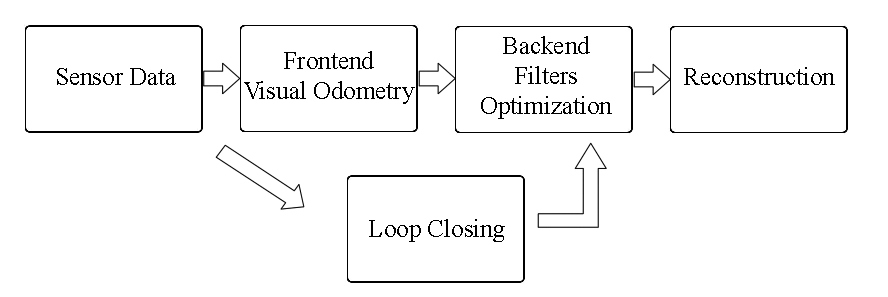
\includegraphics[width=0.8\textwidth]{./resources/whatIsSLAM/workflow.pdf}
    \caption{The classic visual SLAM framework.}
    \label{fig:workflow}
\end{figure}

A typical visual SLAM work-flow includes the following steps:
\begin{enumerate}
\item{Sensor data acquisition}. In visual SLAM, this mainly refers to for acquisition and preprocessing for camera images. For a mobile robot, this will also include the acquisition and synchronization with motor encoders, IMU sensors, etc.
\item{Visual Odometry (VO)}. The task of VO is to estimate the camera movement between adjacent frames (ego-motion), as well as to generate a rough local map. VO is also known as the \emph{Front End}.
\item {Backend filtering/optimization}. The back end receives camera poses at different time stamps from VO, as well as results from loop closing, and apply optimization to generate a fully optimized trajectory and map. Because it is connected after the VO, it is also known as the \emph{Back End}.
\item {Loop Closing}. Loop closing determines whether the robot has returned to its previous position in order to reduce the accumulated drift. If a loop is detected, it will provide information to the back end for further optimization.
\item {Reconstruction}. It constructs a task specific map based on the estimated camera trajectory.
\end{enumerate}

The classic visual SLAM framework is the result of more than a decade's research endeavor. The framework itself and the algorithms have been basically finalized and have been provided as basic functions in several public vision and robotics libraries. Relying on these algorithms, we are able to build visual SLAM systems performing real-time localization and mapping in static environments. Therefore, a rough conclusion can be reached that if the working environment is limited to static and rigid with stable lighting conditions and no human interference, visual SLAM problem is basically solved~\cite{Cadena2016}.

The readers may have not fully understood the concepts of the above mentioned modules yet, so we will detail the functionality of each module in the following sections. However, an deeper understanding of their working principles requires certain mathematical knowledge which will be expanded in the second part of this book. For now, an intuitive and qualitative understanding of each module is good enough.

\subsubsection{Visual Odometry}

The visual odometry is concerned with the movement of a camera between \emph{adjacent image frames}, and the simplest case is of course the motion between two successive images. For example, when we see the images in Fig.~\ref{fig:cameramotion}, we will naturally tell  that the right image should be the result of the left image after a rotation to the left with a certain angle (it will be easier if we have a video input). Let's consider this question: how do we know the motion is ``turning left''? Humans have long been accustomed to using our eyes to explore the world, and estimating our own positions, but this intuition is often difficult to explain, especially in natural language. When we see these images, we will naturally think that, ok, the bar is close to us, the walls and the blackboard are farther away. When the camera turns to left, the closer part of the bar started to appear, and the cabinet on the right side started to move out of our sight. With this information, we conclude that the camera should be be rotating to the left.

\begin{figure}
    \centering
    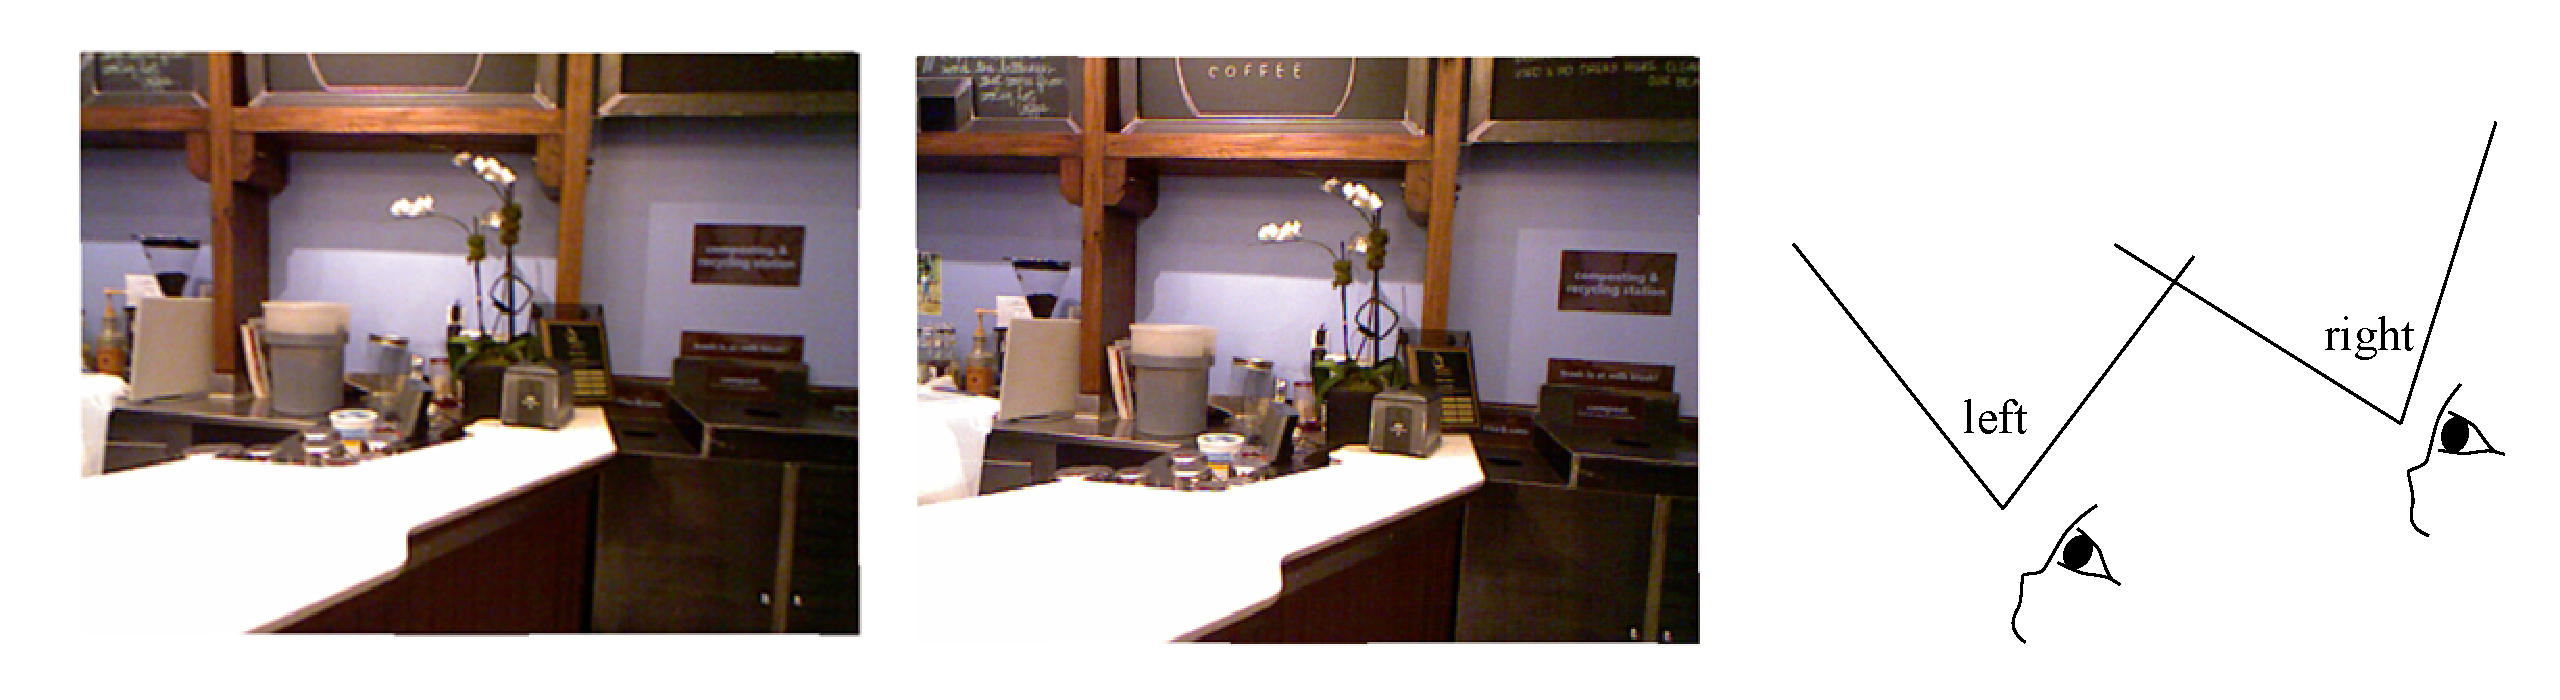
\includegraphics[width=1.0\textwidth]{./resources/whatIsSLAM/cameramotion.pdf}
    \caption{Camera motion can be inferred from two consecutive image frames. Images are from NYUD dataset.}
    \label{fig:cameramotion}
\end{figure}

But if we go a step further: can we determine how much the camera has rotated or translated, in units of degrees or centimeters? It is still difficult for us to give an quantitative answer. Because our intuition is not good at calculating numbers. But for a computer, movements have to be described with such numbers. So we will ask: how should a computer determine a camera's motion only based on images?

As mentioned earlier, in the field of computer vision, a task that seems natural to a human can be very challenging for a computer. Images are nothing but numerical matrices in computers. A computer has no idea what these matrices mean (this is the problem that machine learning is also trying to solve). In visual SLAM, we can only see blocks of pixels, knowing that they are the results of projections by spatial points onto the camera's imaging plane. In order to quantify a camera's movement, we must first \emph{understand the geometric relationship between a camera and the spatial points}.

Some background knowledge is needed to clarify this geometric relationship and the realization of VO methods. Here we only want to convey an intuitive concept. For now, you just need to take away that VO is able to estimate camera motions from images of adjacent frames and restore the 3D structures of the scene. It is named as an ``odometry'', because similar to an actual wheel odometry which only calculates the ego-motion at neighboring moments, and does not estimate a global map or a absolute pose. In this regard, VO is like a species with only a short memory.

Now, assuming that we have a visual odometry, we are able to estimate camera movements between every two successive frames. If we connect the adjacent movements, this constitutes the movement of the robot trajectory, and therefore addresses the positioning problem. On the other hand, we can calculate the 3D position for each pixel according to the camera position at each time step, and they will form an map. Up to here, it seems with an VO, the SLAM problem is already solved. Or, is it?

Visual odometry is indeed an key technology to solving visual SLAM problem. We will be spending a great part to explain it in details. However, using only a VO to estimate trajectories will inevitably cause \emph{accumulative drift}. This is due to the fact that the visual odometry (in the simplest case) only estimates the movement between two frames. We know that each estimate is accompanied by a certain error, and because the way odometry works, errors from previous moments will be carried forward to the following moments, resulting in inaccurate estimation after a period of time (see Fig.~\ref{fig:loopclosure}). For example, the robot first turns left 90$^\circ$ and then turns right 90$^\circ$. Due to error, we estimate the first 90$^\circ$ as 89$^\circ$, which is possible to happen in real-world applications. Then we will be embarrassed to find that after the right turn, the estimated position of the robot will not return to the origin. What's worse, even the following estimates are perfectly estimated, they will always be carrying this 1$^\circ$ error compared to the true trajectory.

\begin{figure}
    \centering
    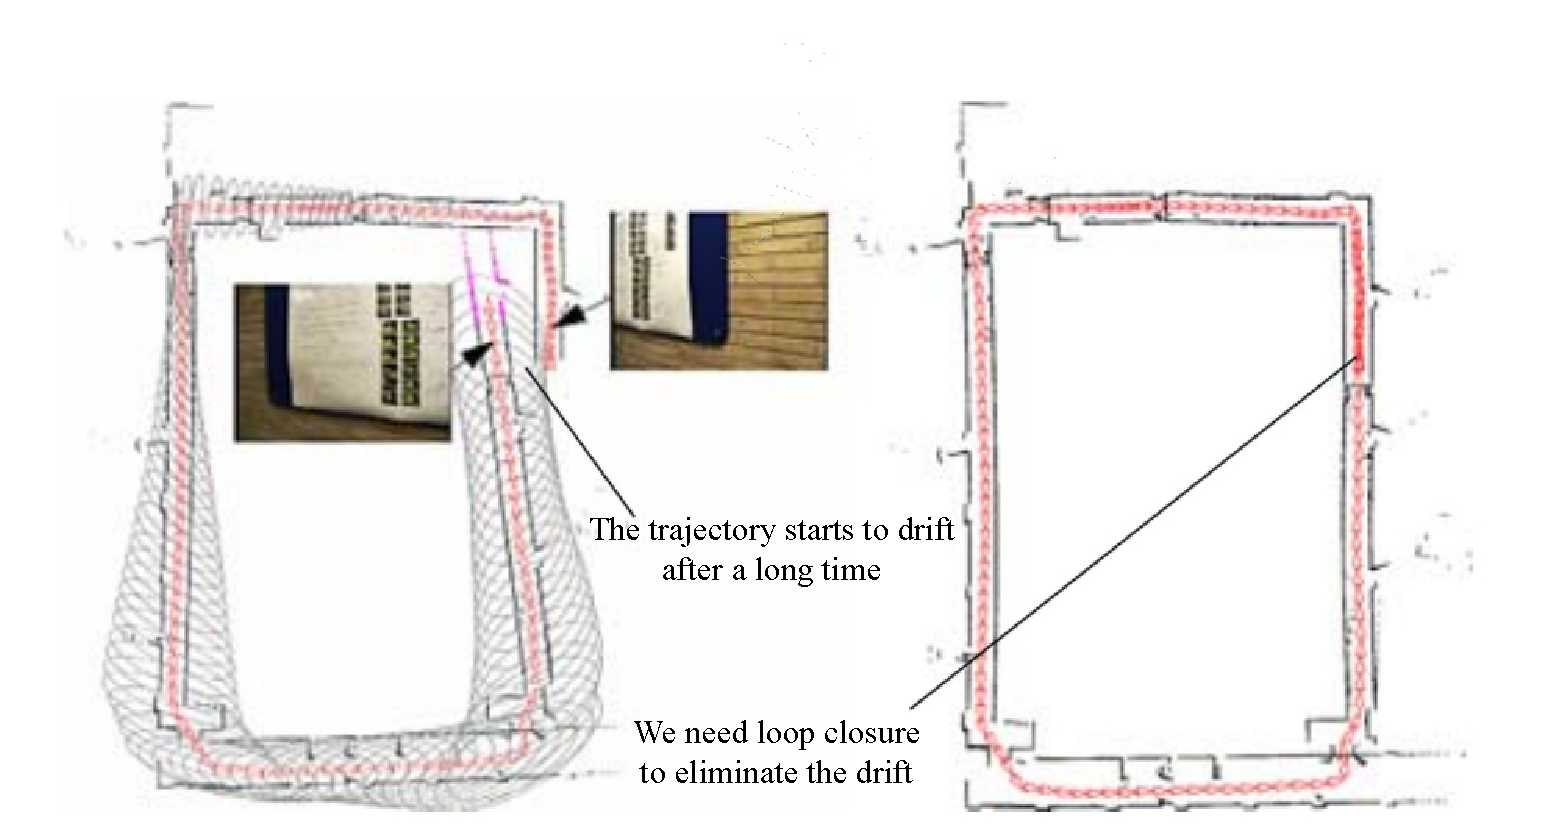
\includegraphics[width=1.0\textwidth]{./resources/whatIsSLAM/loopclosure.pdf}
    \caption{Drift will be accumulated if we only have a relative motion estimation.}
    \label{fig:loopclosure}
\end{figure}

The accumulated drift will make us unable to build a consistent map. A straight corridor may oblique, and a 90$^\circ$ angle may be crooked - this is really an unbearable matter! In order to solve the drifting problem, we also need other two components: the \emph{back-end optimization} \footnote{It is usually known as the back end. Since it is often implemented by optimization so we use the term back-end optimization.} and \emph{loop closing}. Loop closing is responsible for detecting whether the robot returns to its previous position, while the back-end optimization corrects the shape of the entire trajectory based on this information.


\subsubsection{ Back-end Optimization}
Generally speaking, the back-end optimization mainly refers to the process of dealing with the \emph{noise} in SLAM systems. We wish that all the sensor data is accurate, but in reality, even the most expensive sensors still have certain amount of noise. Cheap sensors usually have larger measurement errors, while that of expensive ones may be small. Moreover, performance of many sensors are affected by changes in magnetic field, temperature, etc. Therefore, in addition to solving the problem of estimating camera movements from images, we also care about how much noise this estimation contains, how these noise is carried forward from the last time step to the next, and how confident we have on the current estimation. So the problem that back-end optimization solves can be summarized as: to estimate the state of the entire system from noisy input data and calculate how uncertain these estimations are. The state here includes both the robot's own trajectory and the environment map.

In contrast, the visual odometry part is usually referred to as the \emph{front end}. In a SLAM framework, the front end provides data to be optimized by the back end, as well as the initial values. Because the back end is responsible for the overall optimization, we only care about the data itself instead of where it comes from. In other words, we only have numbers and matricies in backend without those beautiful images. In visual SLAM, the front end is more relevant to \emph{computer vision} topics, such as image feature extraction and matching, while the backend is relevant to \emph{state estimation} research area.

Historically, the back-end optimization part has been equivalent to ``SLAM research'' for a long time. In the early days, SLAM problem was described as a state estimation problem, which is exactly what the back-end optimization tries to solve. In the earliest papers on SLAM, researchers at that time called it ``estimation of spatial uncertainty''~\cite{Smith1986, Smith1990}. Although sounds a little obscure, it does reflect the nature of the SLAM problem: \emph{the estimation of the uncertainty of the self-movement and the surrounding environment}. In order to solve the SLAM problem, we need state estimation theory to express the uncertainty of localization and map construction, and then use filters or nonlinear optimization to estimate the mean and uncertainty (covariance) of the states. The details of state estimation and non-linear optimization will be explained in chapter 6, 10 and 11.

\subsubsection{Loop Closing}
Loop Closing, also known as \emph{Loop Closure Detection}, is mainly to address the drifting problem of position estimation in SLAM. So how to solve it? Assuming that a robot has returned to its origin after a period of movement, but the estimated position does not return to the origin due to drift. How to correct it? Imagine that if there is some way to let the robot know that it has returned to the origin, then we can then ``pull'' the estimated locations to the origin to eliminate drifts, which is, exactly, called loop closing.

Loop closing has close relationship with both localization and map building. In fact, the main purpose of building a map is to enable a robot to know the places it has been to. In order to achieve loop closing, we need to let the robot has the ability to identify the scenes it has visited before. There are different alternatives to achieve this goal. For example, as we mentioned earlier, we can set a marker at where the robot starts, such as a QR code. If the sign was seen again, we know that the robot has returned to the origin. However, the marker is essentially an intrusive sensor which sets additional constraints to the application environment. We prefer the robot can use its non-intrusive sensors, e.g.\ the image itself, to complete this task. A possible approach would be to detect similarities between images. This is inspired by us humans. When we see two similar images, it is easy to identify that they are taken from the same place. If the loop closing is successful, accumulative error can be significantly reduced. Therefore, visual loop detection is essentially an algorithm for calculating similarities of images. Note that the loop closing problem also exists in laser based SLAM, but here the rich information contained in images can remarkably reduce the difficulty of making a correct loop detection.

After a loop is detected, we will tell the back-end optimization algorithm that, OK,  ``A and B are the same point''. Then, based on this new information, the trajectory and the map will be adjusted to match the loop detection result. In this way, if we have sufficient and reliable loop detection, we can eliminate cumulative errors, and get globally consistent trajectories and maps.

\subsubsection{Mapping}
Mapping means the process of building a map, whatever kind it is. A map (see Fig.~\ref{fig:mapping}) is a description of the environment, but the way of description is not fixed and depends on the actual application.

\begin{figure}
	\centering
	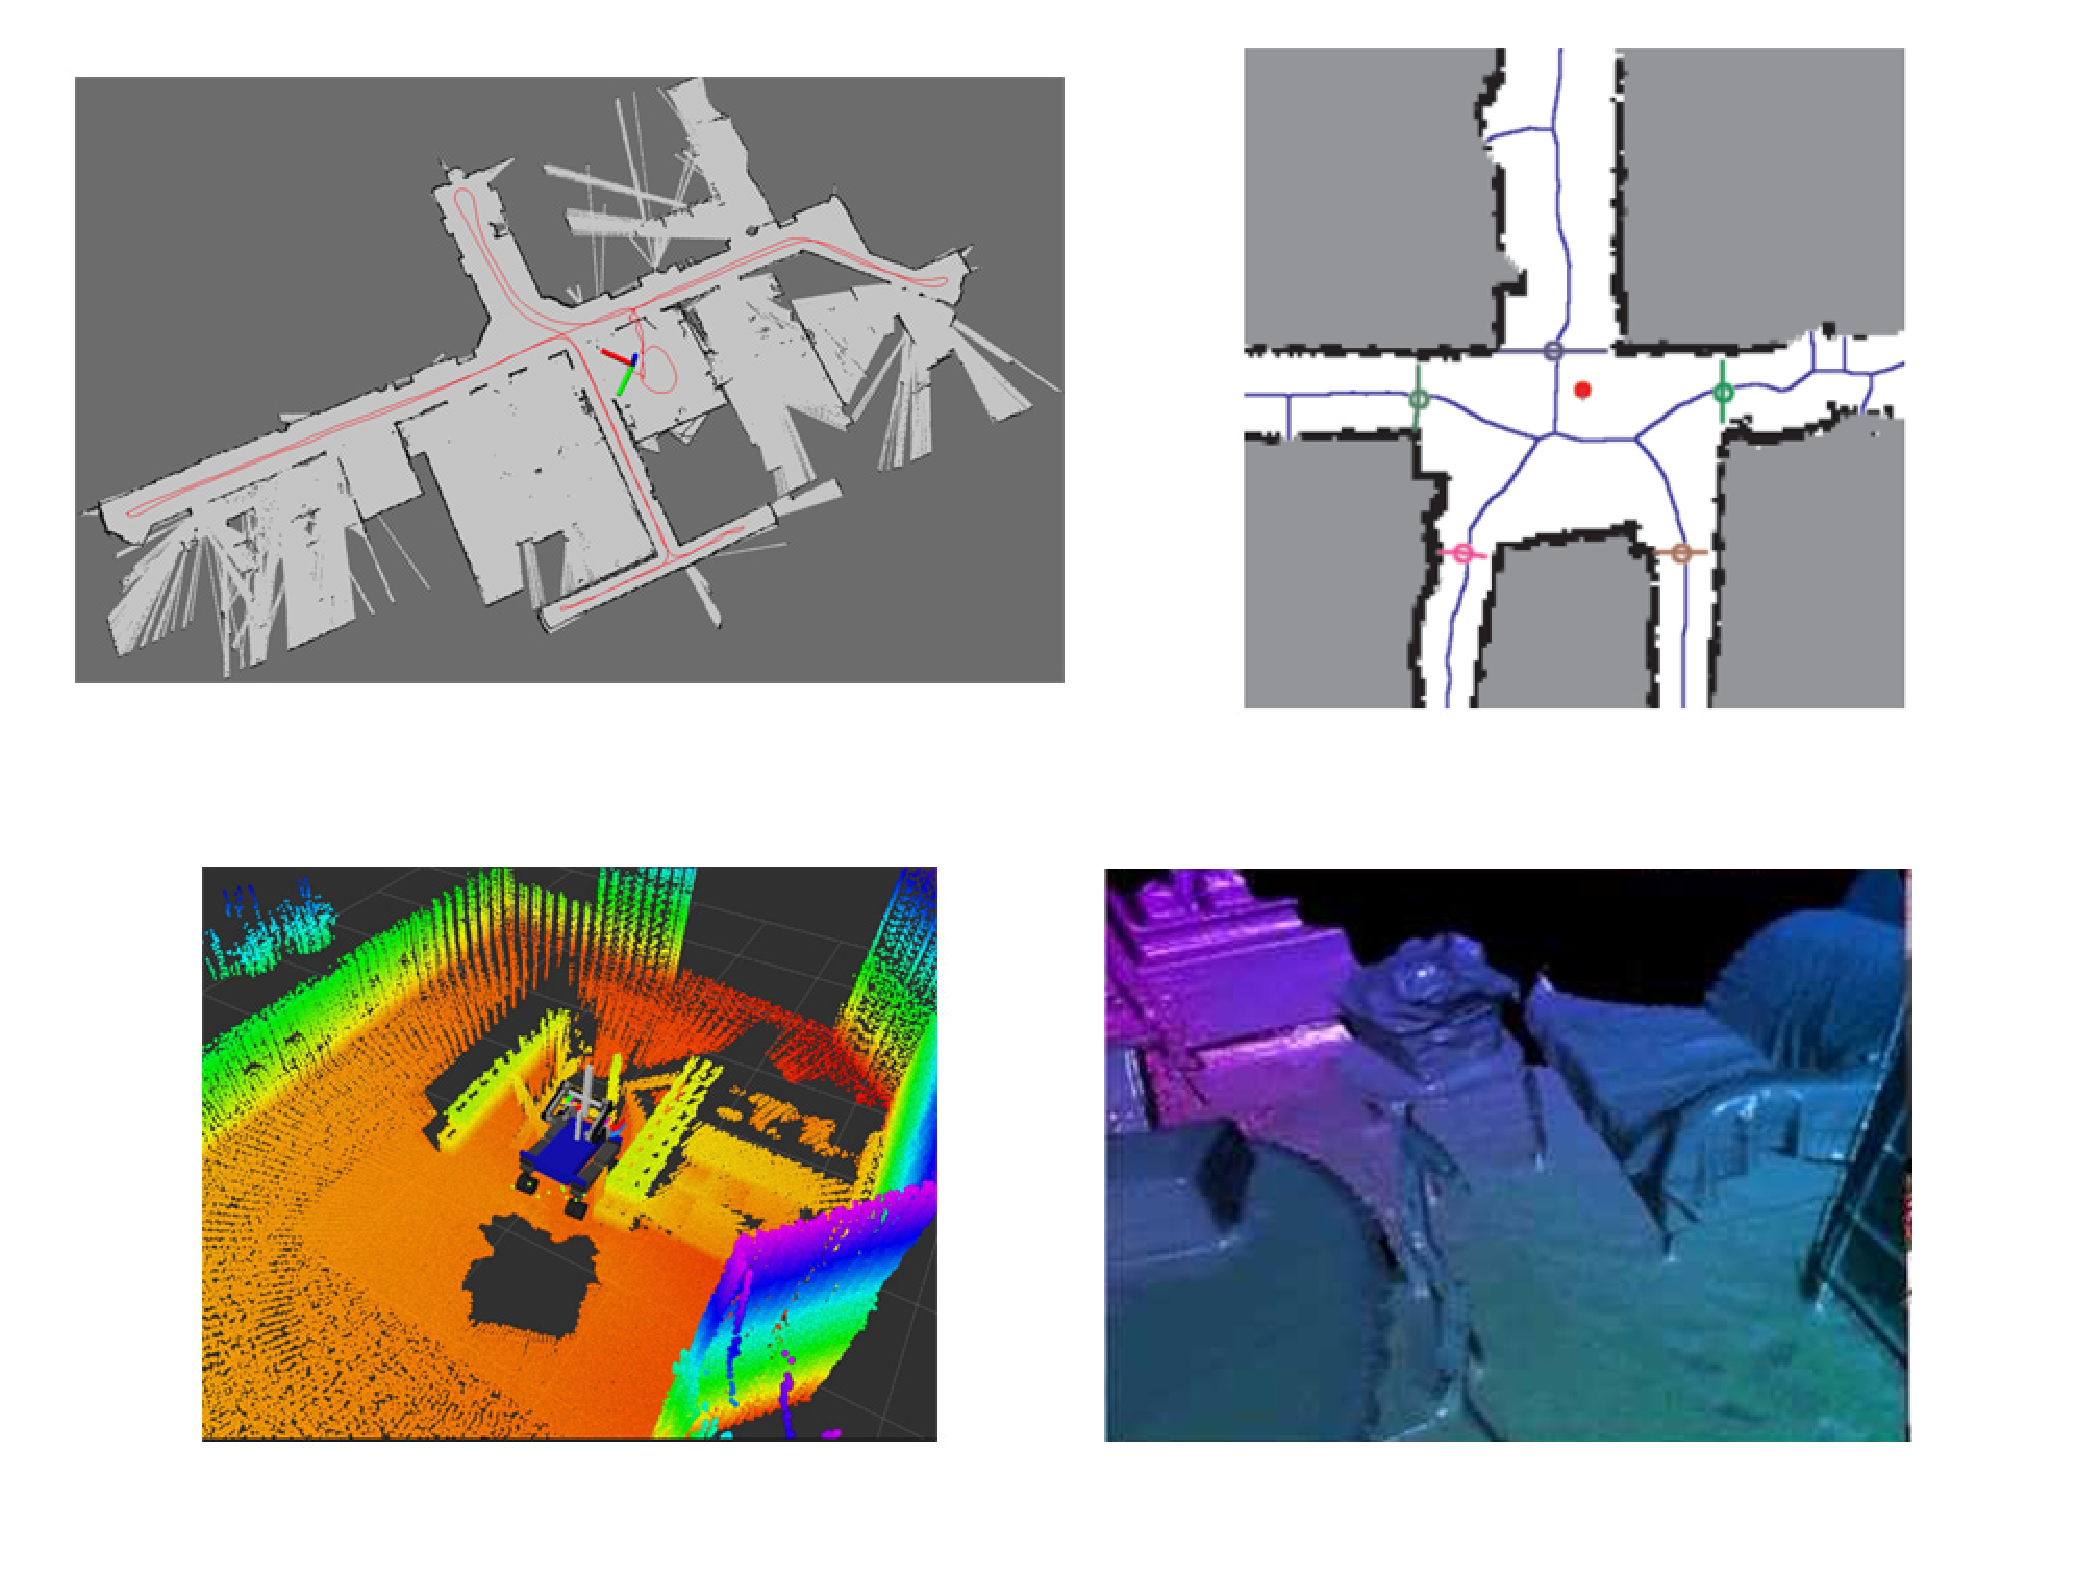
\includegraphics[width=1.0\textwidth]{./resources/whatIsSLAM/map.pdf}
	\caption{Different kinds of maps: 2D grid map, 2D topological map, 3D point clouds and 3D meshes.}
	\label{fig:mapping}
\end{figure}

Let's take the domestic cleaning robots as an example. Since they basically move on the ground, a two-dimensional map with marks for open areas and obstacles, built by a single line laser scanner, would be sufficient for navigation for them. And for a camera, we need at least a three-dimensional map for its 6 degrees of freedom movement. Sometimes, we want a smooth and beautiful reconstruction result, not just a set of points, but also with texture of triangular faces. And at other times, we do not care about the map, just need to know things like ``point A and point B are connected, while point B and point C are not'', which is a topological way to understand the environement. Sometimes maps may not even be needed, for instance, a level-3 autonomous driving car can make a lane-following driving only knowing its relative motion with the lanes.

For maps, we have various ideas and demands. So compared to the previously mentioned VO, loop closure detection and back-end optimization, map building does not have a certain algorithm. A collection of spatial points can be called a map, a beautiful 3D model is also a map, so is a picture of a city, a village, railways, and rivers. The form of the map depends on the application of SLAM. In general, they can be divided into to categories: \emph{metrical map} and \emph{topological map}.

\paragraph{Metric Map}
Metrical maps emphasize the exact metrical locations of the objects in maps. They are usually classified as either sparse or dense. Sparse metric maps store the scene into a compact form, and do not express all the objects. For example, we can construct a sparse map by selecting representative landmarks such as the lanes and traffic signs, and ignore other parts. In contrast, dense metrical maps focus on modeling all the things that are seen. For localization, sparse map would be enough, while for navigation, a dense map is usually needed (otherwise we may hit a wall between two landmarks). A dense map usually consists of a number of small pieces at a certain resolution. It can be small grids for 2D metric maps, or small voxels for 3D maps. For example, in a grid map, an grid may have three states: occupied, idle, and unknown, to express whether there is an object. When a spatial location is queried, the map can give the information about whether the location can be passed through. This type of maps can be used for a variety of navigation algorithms, such as A$^*$, D$^*$\footnote{ See \url{https://en.wikipedia.org/wiki/A*_search_algorithm}.}, etc., and thus attracts the attention of robotics researchers. But we can also see that all the grid status are store in the map, and thus being storage expensive. There are also some open issues in building a metrical map, for example, in large-scale metrical maps, a little bit of steering error may cause the walls of two rooms to overlap with each other, and thus making the map ineffective.

\paragraph{Topological Map}
Compared to the accurate metrical maps, topological maps emphasize the relationships among map elements. A topological map is a graph composed of nodes and edges, only considering the connectivity between nodes. For instance, we only care about that point A and point B are connected, regardless how we could travel from point A to point B. It relaxes the requirements on precise locations of a map by removing map details, and is therefore a more compact expression. However, topological maps are not good at representing maps with complex structures. Questions such as how to split a map to form nodes and edges, and how to use a topological map for navigation and path planning, are still open problems to be studied.

\section{Mathematical Formulation of SLAM Problems}
Through the previous introduction, readers should have gained an intuitive understanding of the modules in a SLAM system and the main functionality of each module. However, we cannot write runable programs only based on intuitive impressions. We want to rise it to a rational and rigorous level, that is, using mathematical symbols to formulate a SLAM process. We will be using variables and formulas, but please rest assured that we will try our best to keep it clear enough.

Assuming that our Little Carrot is moving in an unknown environment, carrying some sensors. How can this be described in mathematical language? First, since sensors usually collect data at different some time points, we are only concerned with the locations and map at these moments. This turns a continuous process into discrete time steps, say $1, \cdots, k$, at which data sampling happens. We use $\mathbf{x}$ to indicate positions of Little Carrot. So the positions at different time steps can be written as $\mathbf{x}_1,\cdots,\mathbf{x}_k$, which constitute the trajectory of Little Carrot. In terms of the map, we assume that the map is made up of a number of \emph{landmarks}, and at each time step, the sensors can see a part of the landmarks and record their observations. Assume there are total $N$ landmarks in the map, and we will use $\mathbf{y}_1, \cdots, \mathbf{y}_N$ to denote them.

With such a setting, the process that ``Little Carrot move in the environment with sensors'' basically has two parts: 

\begin{enumerate}
\item What is its \emph{motion}? We want to describe how $\mathbf{x}$ has changed from time step $k-1$ to $k$.
\item What are the sensor \emph{observations}? Assuming that the Little Carrot detects a certain landmark, let's say $\mathbf{y}_j$ at position $\mathbf{x}_k$, we need to describe this event in mathematical language.
\end{enumerate}

Let's first take a look at motion. Typically, we may send some motion message to the robots like ``turn 15 degree to left''. These messages or orders will be finally carried out by the controller, but probably in may different ways. Sometimes we control the position of robots, but acceleration or angular velocity would always be reasonable alternates. However, no matter what the controller is, we can use a universal and abstract mathematical model to describe it:
\begin{equation}
{\mathbf{x}_k} = f\left( {{\mathbf{x}_{k - 1}},{\mathbf{u}_k}, \mathbf{w}_k} \right),
\end{equation}
where $\mathbf{u}_k$ is the input orders, and $\mathbf{w}_k$ is noise. Note that we use a general $f(\cdot)$ to describe the process, instead of specifying the exact form of $f$. This allows the function to represent any motion input, rather than being limited to a particular one, and thus becoming a general equation. We call it the \emph{motion equation}.

The presence of noise turns this model into a stochastic model. In other words, even if we give the order like ``move forward one meter'', it does not mean that our robot really advances one meter. If all the instructions are accurate, there is no need to \emph{estimate} anything. In fact, the robot may only advance by, say, 0.9 meters, and at another moment, it moves by 1.1 meters. Thus, the noise during each movement is random. If we ignore this noise, the position determined only by the command may be a hundred miles away from the actual position after several minutes.

Corresponding to the motion equation, there is also an \emph{observation equation}. The observation equation describes the process that the Little Carrot sees a landmark point $\mathbf{y}_j$ at $\mathbf{x}_k$ and generates an observation data $\mathbf{z}_{k,j}$. Likewise, we will describe this relationship with an abstract function $h(\cdot)$:
\begin{equation}
{\mathbf{z}_{k,j}} = h\left( {{\mathbf{y}_j},{\mathbf{x}_k}, \mathbf{v}_{k,j} } \right),
\end{equation}
where $\mathbf{v}_{k,j}$ is the noise in this observation. Since there are various forms of observation sensors, the observed data $\mathbf{z}$ and the observation equation $h$ may also have many different forms.

Readers may say that the function $f,h$ here does not seem to specify what is going on in the motion and observation. Also, what does $\mathbf{x}$, $\mathbf{y}$, $\mathbf{z}$ mean here? In fact, depending on the actual motion and the type of sensor, there are several kinds of \textbf{parameterization} methods. What is parameterization? For example, suppose our robot moves in a plane, then its pose \footnote{ In this book, we use the word ``pose'' to mean ``position'' plus ``rotation''. } is described by two $x-y$ coordinates and an angle, ie $\mathbf{x}_k = [x_1,x_2,\theta]_k^\mathrm{T}$, where $x_1, x_2$ are positions on two axes and $\theta$ is the angle. At the same time, the input command is the position and angle change between the time interval: $\mathbf{u}_k = [ \Delta x_1, \Delta x_2, \Delta \theta ]_k^\mathrm{T} $, so the motion equation can be parameterized as:
\begin{equation}
{\left[ \begin{array}{l}
    x_1\\
    x_2\\
    \theta
    \end{array} \right]_k} = {\left[ \begin{array}{l}
    x_1\\
    x_2\\
    \theta
    \end{array} \right]_{k - 1}} + {\left[ \begin{array}{l}
    \Delta x_1\\
    \Delta x_2\\
    \Delta \theta
    \end{array} \right]_k} + {\mathbf{w}_k},
\end{equation}
where $\mathbf{w}_k$ is the noise again. This is a simple linear relationship. However, not all input commands are position and angular changes. For example, the input of ``throttle'' or ``joystick'' is the speed or acceleration, so there are other forms of more complex equations of motion. At that time, we would say the kinetic analysis is required.

Regarding the observation equation, for example, the robot carries a two-dimensional laser sensor. We know that when a laser sensor observes a 2D landmark by measuring two quantities: the distance $r$ between the landmark point and the robot, and the angle $\phi$. Let's say the landmark is at $\mathbf{y}_j = [y_1, y_2]_j^\mathrm{T}$, the pose is $\mathbf{x}_k=[x_1,x_2]_k^\mathrm{T}$,and the observed data is $\mathbf{z}_{k,j} = [r_{k,j}, \phi_{k,j}]^\mathrm{T}$, then the observation equation is written as:
\begin{equation}
\left[ \begin{array}{l}
r_{k,j}\\
\phi_{k,j}
\end{array} \right] = \left[ \begin{array}{l}
\sqrt {{{\left(y_{1,j} - x_{1,k} \right)}^2} + {{\left( {{y_{2,j}} - x_{2,k} } \right)}^2}} \\
\arctan \left( \frac{{y_{2,j}} - x_{2,k}}{{y_{1,j} - x_{1,k}}} \right)
\end{array} \right] + \mathbf{v}_{k, j}.
\end{equation}

When considering about visual SLAM, the sensor is a camera, then the observation equation is a process like ``getting the pixels in the image of the landmarks.'' This process involves a description of the camera model, which will be covered in detail in Chapter 5, which is skipped here.

Obviously, it can be seen that the two equations have different parameterized forms for different sensors. If we maintain versatility and take them into a common abstract form, then the SLAM process can be summarized into two basic equations:
\begin{equation}
\label{eq:slamproblem}
\left\{ \begin{array}{l}
{\mathbf{x}_k} = f\left( {{\mathbf{x}_{k - 1}},{\mathbf{u}_k}}, \mathbf{w}_k \right),\quad k=1,\cdots, K\\
{\mathbf{z}_{k,j}} = h\left( {{ \mathbf{y}_j},{ \mathbf{x}_k}}, \mathbf{v}_{k,j} \right), \quad (k,j) \in \mathcal{O}
\end{array} \right. ,
\end{equation}
where $\mathcal{O}$ is a set that contains the information at which pose the landmark was observed (usually not all the landmarks can be seen at every moment – ​​we are likely to see only a small part of the landmarks  at a single moment). These two equations together describe a most basic SLAM problem: how to solve the estimate $\mathbf{x}$ (localization) and $\mathbf{y}$ (mapping) problem with the noisy control input $\mathbf{u}$ and the sensor reading $\mathbf{z}$ data? Now, as we see, we have modeled the SLAM problem as a \textbf{state estimation problem}: How to estimate the internal, hidden state variables through the noisy measurement data?

The solution to the state estimation problem is related to the specific form of the two equations and which distribution the noise obeys. According to whether the motion and observation equations are \textbf{linear}, and whether the noise is assumed to be \textbf{Gaussian}, it is divided into \textbf{linear/nonlinear} and \textbf{Gaussian/non-Gaussian} systems. The Linear Gaussian (LG system) is the simplest, and its unbiased optimal estimation can be given by the Kalman Filter (KF). In the complex nonlinear non-Gaussian (NLNG system), we basically rely on two methods: Extended Kalman Filter (EKF) and nonlinear optimization. Until the early 21st century, the EKF-based filter method still dominated SLAM. We will linearize the system at the working point and solve it in two steps: predict-update (see Lecture 10). The earliest real-time visual SLAM system was developed based on EKF {\cite{Davison2007}}. Subsequently, in order to overcome the shortcomings of EKF (such as the linearization error and noise Gaussian distribution assumptions), people began to use other filters such as particle filters, and even use nonlinear optimization methods. Today, the mainstream of visual SLAM uses state-of-the-art optimization techniques represented by Graph Optimization {\cite{Strasdat2012}}. We believe that optimization methods are clearly superior to filters, and as long as computing resources allow, optimization methods are often preferred (see lectures 10 and 11).

Now we believe the reader has a general understanding of the mathematical model of SLAM, but we still need to clarify some issues. First, we should explain what the \textbf{pose} $\bm{x}$ is. The word \textbf{pose} we just said is somewhat vague. Perhaps the reader can understand that a robot moving in the plane can be parameterized by two coordinates plus an angle. However, more robots are more like things in the three-dimensional space. We know that the motion of the three-dimensional space consists of three axes, so the movement of the robot is described by the translation on the three axes and the rotation around the three axes, totally having six Degrees of Freedom (DoF). But wait, does that mean that we can describe it with a vector in $\mathbb{R}^6$? We will find that things are not that simple. For a 6 DoF \textbf{pose}\footnote{We will call it \textbf{pose} in the future to distinguish it from the position. The pose we are talking about includes \textbf{Rotation} and \textbf{Translation}. }, how to express it? How to optimize it? How to describe its mathematical properties?  This will be the main content of the third and fourth chapters. Next, we will explain how the \textbf{observation equation} is parameterized in the visual SLAM. In other words, how the landmark points in space are projected onto a photo? This requires an explanation of the camera's projection model and distortion, which we will cover in chapter 5. Finally, when you know this information, \textbf{how to solve the above state estimation problem}? This requires knowledge of nonlinear optimization and is the content of Lecture 6.
    
These contents form part of the mathematical knowledge of this book. After laying the groundwork for them, we can discuss more detailed knowledge of visual odometry, back-end optimization, and more. It can be seen that the content of this lecture constitutes a summary of the book. If you don't understand the above concepts well, you may want to go back and read them again. Let's start the introduction of  programming!


\section{Practice: Basics}
\subsection{Installing Linux}
Finally we come to the exciting practice session! Are you ready? In order to complete the practice of this book, we need to prepare a computer. You can use a laptop or desktop, preferably your personal computer, because we need to install an operating system on it for experiments.

Our program is based on C++ programs on Linux. During the experiment, we will use a number of open source libraries. Most libraries are only supported in Linux, while configuration on Windows is relatively (or quite) cumbersome. Therefore, we have to assume that you already have a basic knowledge of Linux (see the exercises in the previous lecture), including using basic commands to understand how the software is installed. Of course, you don't have to know how to develop C++ programs under Linux, which is exactly what we want to talk about below.

Let's start from installing the experimental environment required for this book. As a book for beginners, we use Ubuntu as a development environment. Ubuntu and its variances have enjoyed a good reputation as a novice user in all major Linux distributions. Ubuntu is an open source operating system. Its system and software can be downloaded freely on the official website (\url{http://ubuntu.com}), which provides detailed instructions on how to install it. At the same time, Tsinghua University, China Science and Technology University and other major universities in China have also provided Ubuntu software mirrors, making the software installation very convenient (probably there are also mirror websites in your country).

The first version of this book uses Ubuntu 14.04 as the default development environment. In the second edition, we updated the default version to the newer \textbf{Ubuntu 18.04} (\autoref{fig:ubuntu1804}) for later research. If you want to change the styles, then Ubuntu Kylin, Debian, Deepin and Linux Mint are also good choices. I promise that all the code in the book has been well tested under Ubuntu 18.04, but if you choose a different distribution, I am not sure if you will encounter some minor problems. You may need to spend some time solving small issues (but you can also take them as opportunities to exercise yourself). In general, Ubuntu's support for various libraries is relatively complete, and the software is also very rich. Although we don't limit which Linux distribution you use, in the explanation, \textbf{we will use Ubuntu 18.04 as an example}, and mainly use Ubuntu commands (such as apt-get), so in other versions of Ubuntu there will be no obvious differences below. In general, the migration of programs between Linux is not very difficult. But if you want to use the programs in this book under Windows or OS X, you need to have some porting experience.

\begin{figure}[!ht]
    \centering
    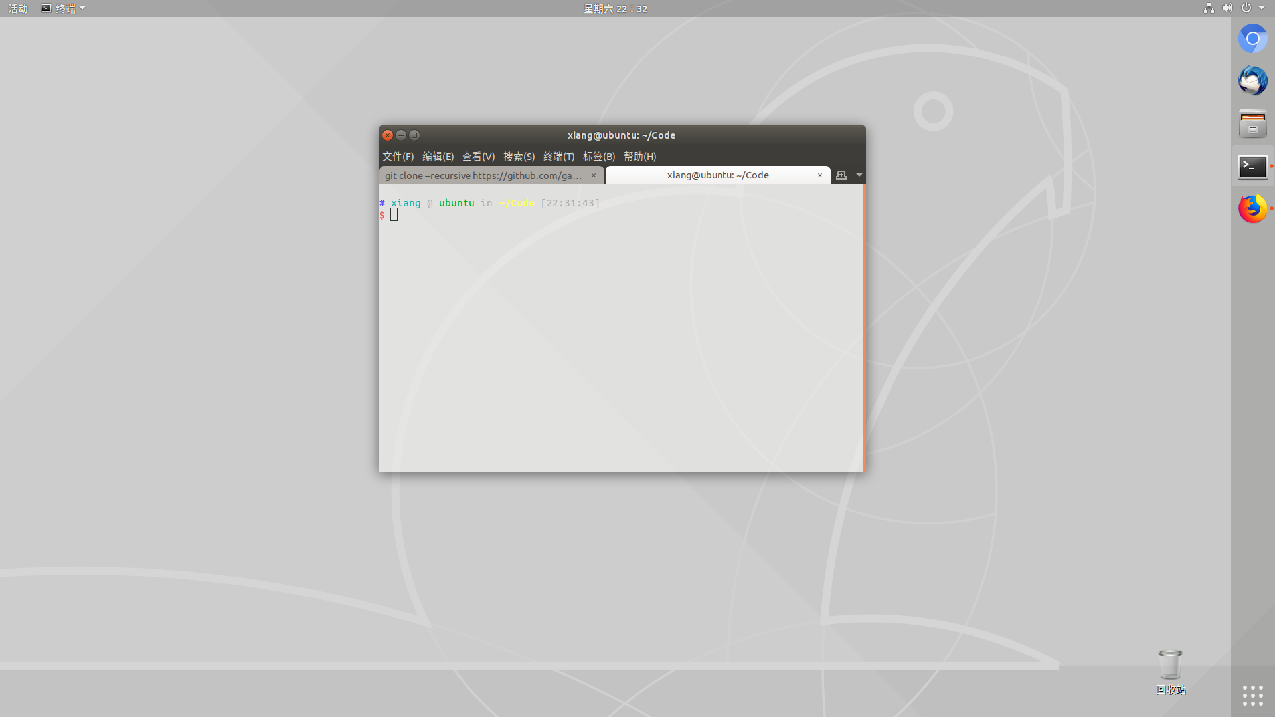
\includegraphics[width=0.8\textwidth]{whatIsSLAM/ubuntu1804.pdf}
    \caption{Ubuntu 1804 in virtual machine.}
    \label{fig:ubuntu1804}
\end{figure}

Now, I assume there's an Ubuntu 18.04 installed on your PC. Regarding the installation of Ubuntu, you can find a lot of tutorials on the Internet. Just do it, I'll skip here. The easiest way is to use a virtual machine (see \autoref{fig:ubuntu1804}), but it takes a lot of memory (our experience is more than 4GB) and CPU to be smooth. You can also install dual systems, which will be faster, but a blank USB flash drive is required as the boot disk. In addition, virtual machine software support for external hardware is often not good enough. If you want to use real sensors (binocular cameras, Kinects, etc.), it is recommended that you use dual systems to install Linux.

Now, let's say you have successfully installed Ubuntu, either it's a virtual machine or a dual system. If you are not familiar with Ubuntu, try its various software and experience its interface and interaction mode\footnote{Most people think Ubuntu is cool for the first time. }. But I have to \textbf{remind} you, especially to the novice friends: don't spend too much time on Ubuntu's user interface! Linux has a lot of chances to waste your time, you may find some niche software, some games, and even spend a lot of time looking for a wallpaper. But remember, you are working with Linux. Especially in this book, you are using Linux to learn SLAM, so try to spend your time on learning SLAM.

Ok, let's choose a directory and put the code for the SLAM program in this book. For example, you can put the code under ``slambook2'' in the home directory (/home). We will refer to this directory as ``\textbf{code root}'' in the future. At the same time, you can choose another directory to copy the Git code of this book, which is convenient for comparison when doing experiments. The code for this book is divided into chapters. For example, the code for this chapter will be under slambook2/ch2, and the next one will be under slambook2/ch3. So, now please go into the slambook2/ch2 directory (you should create a new folder and enter the folder name).

\subsection{Hello SLAM}
Like many computer books, let's write a \textit{HelloSLAM} program. But before we do this, let's talk about what a program is.

In Linux, a program is a file with execute permissions. It can be a script or a binary file, but we don't limit its suffix name (unlike Windows, you need to specify it as an .exe file). The commonly used binaries such as \textbf{cd} and \textbf{ls} are executable files located in the /bin directory. For an executable program elsewhere, as long as it has executable permissions, it will run when we enter the program name in the terminal. When programming in C++, we first write a text file:

\begin{lstlisting}[language=C++,caption=slambook2/ch2/helloSLAM.cpp]
#include <iostream>
using namespace std;

int main(int argc, char **argv) {
    cout << "Hello SLAM!" << endl;
    return 0;
}
\end{lstlisting}

Then use a program called \textbf{compiler} to compile this text file into an executable program. Obviously this is a very simple program which just prints a hello slam text. You should be able to understand it effortlessly, so there is no explanation here - if this is not the case, please take a look at the basics of C++. This program just outputs a string to the screen. You can use the text editor like \textbf{gedit} (or \textbf{Vim}, if you have learned Vim in the previous tutorial) and enter the code and save it in the path listed above. Now, we compile it into an executable using the compiler g++ (g++ is a C++ compiler). Enter:

\begin{lstlisting}[language=sh,caption=Terminal input:]
g++ helloSLAM.cpp
\end{lstlisting}

If it goes well, this command should have no output. If the ``command not found'' error message appears on the screen, you may not have g++ installed yet. Please use the following command to install it:
\begin{lstlisting}[language=sh,caption=terminal input:]
sudo apt-get install g++
\end{lstlisting}
If there are other errors, please check again if the program you just entered is correct.

Just now this compile command compiles the text file helloSLAM.cpp into an executable program. We check the current directory and find that there is an additional a.out file, and it has execute permissions (the colors in the terminal are different, should be green in default settings). We can enter ./a.out to run the program \footnote{Don't type the first \%. }:

\begin{lstlisting}[language=sh,caption=terminal input:]
% ./a.out
Hello SLAM!
\end{lstlisting}

As we thought, this program outputs ``Hello SLAM!'', telling us that it is running correctly.

Please review what we did before. In this example, we used the editor to enter the source code for helloSLAM.cpp, then called the g++ compiler to compile it and get the executable. By default, g++ compiles the source file into a program of the name a.out (it is a bit weird, but acceptable). If we like, we can also specify the file name of this output. This is an extremely simple example, we actually \textbf{use a lot of hidden default parameters, almost omitting all intermediate steps}, in order to give the reader a simple impression (although you may not have realized it). Below we will use cmake to compile this program.

\subsection{Use cmake}
Theoretically, any C++ program can be compiled with g++. But when the program size is getting bigger and bigger, a project may have many folders and source files, and the compiled commands will be longer and longer. Usually a small C++ project may contain more than a dozen classes, and there are complex dependencies between these classes. Some of them are compiled into executables, and some are compiled into libraries. If we only rely on the g++ command, we need to enter a lot of commands, and the whole compilation process will become very cumbersome. Therefore, for C++ projects, using some engineering management tools is more efficient. In history, engineers used \textbf{makefile} to compile automatically, but the cmake to be discussed below is more convenient than it. And cmake is widely used in engineering, we will see that most of the libraries mentioned later use cmake to manage the source code.

In a cmake project, we will use the cmake command to generate a makefile, and then use the make command to compile the entire project based on the contents of the makefile. The reader may not know what a makefile is, but it doesn't matter, we will learn by example. Still taking the above helloSLAM.cpp as an example, this time we are not using g++ directly, but using cmake to build a project and then compiling it. Create a new CMakeLists.txt file in slambook2/ch2/ with the following contents:
\begin{lstlisting}[language=Python,caption=slambook2/ch2/CMakeLists.txt]
cmake_minimum_required( VERSION 2.8 )
project( HelloSLAM )
add_executable( helloSLAM helloSLAM.cpp )
\end{lstlisting}

The CMakeLists.txt file is used to tell cmake what we want to do with the files in this directory. The contents of the CMakeLists.txt file need to follow the cmake syntax. In this example, we demonstrate the most basic project: specifying a project name and an executable program. According to the comments, the reader should understand what each sentence does.

Now, in the current directory (slambook2/ch2/), call cmake to compile the project: \footnote{Note that there's a dot at the end of the command, please don't forget it, which means using cmake in the current directory. }:
\begin{lstlisting}[language=sh,caption=Terminal input]
cmake .
\end{lstlisting}
cmake will output some compilation information, and then generate some intermediate files in the current directory, the most important of which is the makefile\footnote{Makefile is an automated compilation script, the reader can now understand it as a system automatically generated compiler instructions, without taking care of its content. }. Since MakeFile is automatically generated, we don't have to modify it. Now, compile the project with the make command.
\begin{lstlisting}[language=sh,caption=Terminal input]
% make
Scanning dependencies of target helloSLAM
[100%] Building CXX object CMakeFiles/helloSLAM.dir/helloSLAM.cpp.o
Linking CXX executable helloSLAM
[100%] Built target helloSLAM
\end{lstlisting}
The compiler will show a process percent during compilation. We then get the declared executable \textbf{helloSLAM} in our CMakeLists.txt if the compilation is successful. Just type:
\begin{lstlisting}[language=sh,caption=Terminal Input]
% ./helloSLAM
Hello SLAM!
\end{lstlisting}
to run it. Because we didn't modify the source code, we got the same result as before. Please think about the difference between this practice and the previous use of g++ compiler. This time we used the cmake-make process. The cmake process handles the relationship between the project files, and the make process actually calls g++ to compile the program. By calling this cmake-make process, we have a good management for the project: \textbf{from inputting a string of g++ commands to maintaining several relatively intuitive CMakeLists.txt files}, which will obviously reduce the difficulty of maintaining the entire project. For example, if you want to add another executable file, just add a line ``add\_executable'' in CMakeLists.txt, and the subsequent steps are unchanged. Cmake will help us resolve code dependencies without having to type in a bunch of g++ commands.

The only thing that is dissatisfied with this process is that the intermediate files generated by cmake are still in our code files. When we want to release the code, we don't want to publish these intermediate files together. At this time, we still need to delete them one by one, which is very inconvenient. A better approach is to have these intermediate files in an intermediate directory. After the compilation is successful, we will delete the intermediate directory. Therefore, the more common practice of compiling cmake projects is as follows:
\begin{lstlisting}[language=sh,caption=Terminal input]
mkdir build
cd build
cmake ..
make
\end{lstlisting}
We created a new intermediate folder ``build'', and then entered the build folder, using the cmake .. command to compile the previous folder, which is the folder where the code is located. In this way, the intermediate files generated by cmake will be in the ``build'' folder, separate from the source code. When publishing the source code, we just delete the build folder. Please try to compile the code in ch2 in this way, and then call the generated executable (please remember to delete the intermediate file generated in the last section).

\subsection{Use Libraries}
In a C++ project, not all code is compiled into executables. Only executable files with the main function will generate executable programs. For other code, we just want to package them into a packet for other programs to call. This packet is called \textbf{library}.

A library is often just a collection of many algorithms and programs, and we will be exposed to many libraries in later exercises. For example, the OpenCV library provides many computer vision related algorithms, while the Eigen library provides calculations of matrix algebra. Therefore, we need to learn how to use cmake to generate libraries and use the functions in the library. Now let's demonstrate how to write a library yourself. Write the following libHelloSLAM.cpp file:

\begin{lstlisting}[language=c++,caption=slambook2/ch2/libHelloSLAM.cpp]
#include <iostream>
using namespace std;

// Just a function printing hello message
void printHello() {
    cout << "Hello SLAM" << endl;
}
\end{lstlisting}
This library provides a printHello function that will output a message. But it doesn't have a main function, which means there are no executables in this library. We add the following to CMakeLists.txt:
\begin{lstlisting}[language=sh,caption=slambook2/ch2/CMakeLists.txt]
add_library( hello libHelloSLAM.cpp )
\end{lstlisting}
This line tells cmake that we want to compile this file into a library called ``hello''. Then, as above, compile the entire project using cmake:
\begin{lstlisting}[language=sh,caption=Terminal input]
cd build
cmake ..
make
\end{lstlisting}
At this point, a libhello.a file is generated in the build folder, which is the library we declared.

In Linux, the library files are divided into \textbf{static library} and \textbf{shared library}. Static libraries have a .a extension and shared libraries end with .so. All libraries are collections of functions that are packaged. The difference is that \textbf{a static library will generate a copy each time it is called, and the shared library has only one copy}, which saves space. If you want to generate a shared library instead of a static library, just use the following statement:

\begin{lstlisting}[language=sh,caption=slambook2/ch2/CMakeLists.txt]
add_library( hello_shared SHARED libHelloSLAM.cpp )
\end{lstlisting}
Then we will get a libhello\_shared.so.

The library file is a compressed package with compiled binary functions. However, if there is only a .a or .so library file, then we don't know what the function is and how to call it. In order for others (or ourselves) to use this library, we need to provide a \textbf{header file} to indicate what is in the library. Therefore, for the user of the library, \textbf{you can call this library as long as you get the header and library files}. Write the header file for libhello below.

\begin{lstlisting}[language=c++,caption=slambook2/ch2/libHelloSLAM.h]
#ifndef LIBHELLOSLAM_H_
#define LIBHELLOSLAM_H_

// Declares a function in header file
void printHello();

#endif
\end{lstlisting}

In this way, according to this file and the library file we just compiled, you can use the printHello function. Finally, we write an executable program to call this simple function:

\begin{lstlisting}[language=c++,caption=slambook2/ch2/useHello.cpp]
#include "libHelloSLAM.h"

// Call printHello() in libHelloSLAM.h
int main(int argc, char **argv) {
    printHello();
    return 0;
}
\end{lstlisting}

Then, declare an executable in CMakeLists.txt and \textbf{link} it to the library: 
\begin{lstlisting}[caption=slambook2/ch2/CMakeLists.txt]
add_executable( useHello useHello.cpp )
target_link_libraries( useHello hello_shared )
\end{lstlisting}

Through these two lines of statements, the useHello program can successfully use the code in the hello\_shared library. This small example demonstrates how to generate and call a library. Please note that for libraries provided by others, we can also call them in the same way and integrate them into our own programs.

In addition to the features already demonstrated, cmake has many more syntax and options. Of course we can not list all of them here. In fact, cmake is very similar to a normal programming language, with variables and conditional control statements, so you can learn cmake just like learning programming. The exercises contain some reading materials for cmake, which can be read by interested readers. Now, a brief review of what we did before:

\begin{enumerate}
    \item First, the program code consists of a header file and a source file.
    \item The source file with the main function is compiled into an executable program, and the other is compiled into a library file.
    \item If the executable wants to call a function in the library file, it needs to refer to the header file provided by the library to understand the format of the call. Also, link the executable to the library file.
\end{enumerate}

These steps should be simple and clear, but you may encounter some problems in the actual operation. For example, what happens if the executable references a library function but we forget to link the library? Try removing the link command in CMakeLists.txt and see what happens. Can you understand the error message reported by cmake?

\subsection{Use IDE}
Finally, let's talk about how to use the Integrated Development Environments (IDEs). The previous programming can be done with a simple text editor. However, you may need to jump between files to query the declaration and implementation of a function. This can be a little annoying when there are too many files. The IDE provides developers with a lot of convenient functions such as jump, completion, breakpoint debugging, etc. Therefore, we recommend that the reader choose an IDE for development.

There are many kinds of IDEs under Linux. Although there are still some gaps with the best IDE (I mean Visual Studio in Windows), there are several supported C++ developments, such as Eclipse, Qt Creator, Code::Blocks, Clion, Visual Studio Code, and so on. Again, we don't force readers to use a particular IDE, but only give our advice. We are using KDevelop and Clion (see \autoref{fig:kdevelop} and \autoref{fig:clion})\footnote{However, the recent Visual Studio Code is getting better and better. It's free. It's very popular among developers. You may have a try. }. KDevelop is a free software located in Ubuntu's software repository, meaning you can install it with apt-get; Clion is a paid software, but you can use the student mailbox for free for one year. Both are good C++ development environments, the advantages are listed below:

\begin{enumerate}
    \item Support cmake projects.
    \item Support C++ better (including the 11 and later standards). There are highlighting, jumping, and finishing functions. Can automatically format the code.
    \item Makes it easy to see individual files and directory trees.
    \item Has one-click compilation, breakpoint debugging and other functions.
\end{enumerate}

\begin{figure}[!ht]
    \centering
    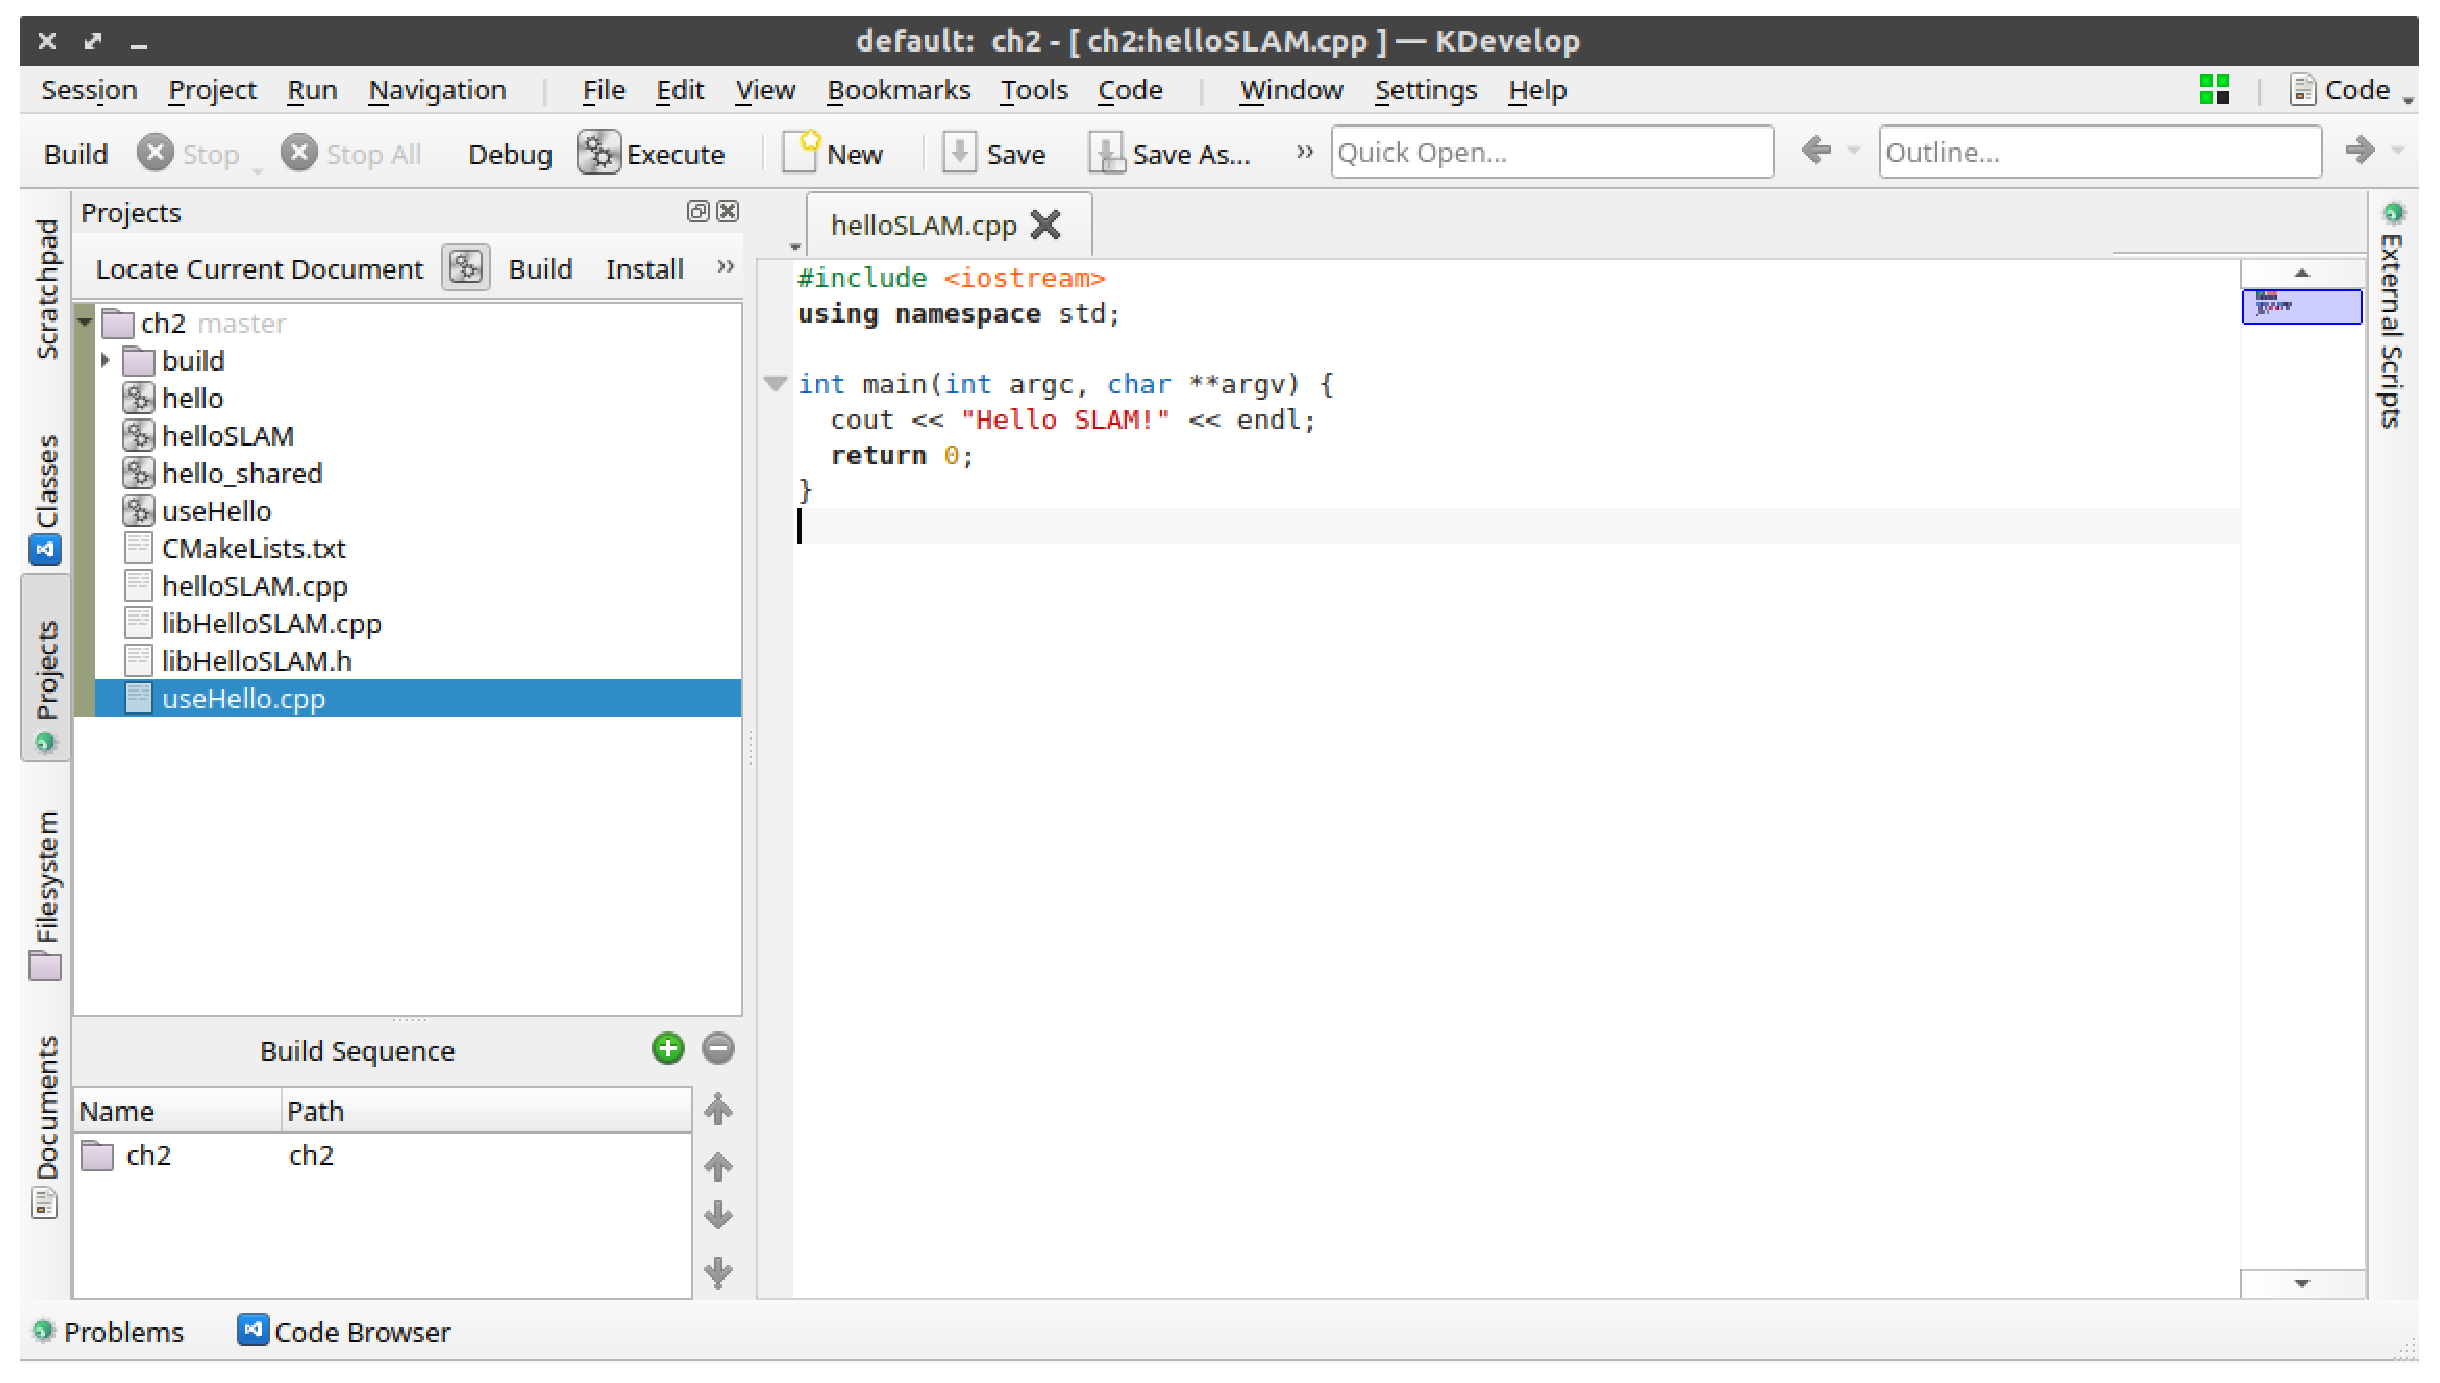
\includegraphics[width=0.8\textwidth]{whatIsSLAM/kdevelop.pdf}
    \caption{Kdevelop in Ubuntu.}
    \label{fig:kdevelop}
\end{figure}

Below we take a little bit of space to introduce KDevelop and Clion.

\subsubsection{Use KDE}
Kdevelop natively supports the cmake project. To do this, after creating CMakeLists.txt in the terminal, open CMakeLists.txt with ``Project $\rightarrow$Open/Import Project'' in KDevelop. The software will ask you a few questions, and by default create a build folder to help you call the cmake and make commands. These can be done automatically by pressing the shortcut key F8. The following section of \autoref{fig:kdevelop} shows the compilation information.

We hand over the task of adapting to the IDE to the reader. If you are transferring from Windows, you will find its interface similar to Visual C++ or Visual Studio. Please use KDevelop to open the previous project and compile it to see what information it outputs. I believe you will feel more convenient than opening the terminal.

Next, let's show to debug in the IDE. Most of the students who program under Windows will have experience of breakpoint debugging under Visual Studio. However, in Linux, the default debugging tool gdb only provides a text interface, which is not convenient for novices. Some IDEs provide breakpoint debugging (the bottom layer is still gdb), and KDevelop is one of them. To use KDevelop's breakpoint debugging feature, you need to do the following:

\begin{enumerate}
    \item Set the project to Debug compilation mode in CMakeLists.txt, and don't use optimization options (not used by default).
    \item Tell KDevelop which program you want to run. If there are parameters, also configure its parameters and working directory.
    \item Enter the breakpoint debugging interface, you can single step, see the value of the intermediate variable.
\end{enumerate}

%\clearpage

The first step is to set the compilation mode by adding the following command to CMakeLists.txt:
\begin{lstlisting}[caption=slambook2/ch2/CMakeLists.txt]
Set( CMAKE_BUILD_TYPE "Debug" )
\end{lstlisting}

Cmake has some compilation-related built-in variables that give you more detailed control over the compilation process. For the compilation type, there is usually a Debug mode for debugging and a Release mode for publishing. In Debug mode, the program runs slower, but breakpoint debugging is possible, and you can see the values of the variables; while Release mode is faster, but there is probably no debugging information. We set the program to Debug mode and place the breakpoint. Next, tell KDevelop which program you want to launch.

In the second step, open ``Run $\rightarrow$Configure Launcher'' and click on ``Add New $\rightarrow$ Application'' on the left. In this step, our task is to tell KDevelop which program to launch. As shown in \autoref{fig:launchConfigure}, you can either select a cmake project target (that is, the executable we built with the add\_executable directive) or point to a binary file. The second approach is recommended, and in our experience, this is less of a problem.

\begin{figure}[!ht]
    \centering
    \includegraphics[width=0.8\textwidth]{whatIsSLAM/launchConfigure.pdf}
    \caption{Config launches. We can choose a launch target and set parameters here. }
    \label{fig:launchConfigure}
\end{figure}

In the second column, you can set the program's parameters and working directory. Sometimes programs have runtime parameters that are passed in as arguments to the main function. If not, leave it blank, as is the working directory. After configuring these two items, click the ``OK'' button to save the configuration results.

In just these steps we have configured an application startup item. For each startup item, we can click the ``Execute'' button to start the program directly, or click the ``Debug'' button to debug it. Readers can try to click the ``Execute'' button to see the results of the output. Now, to debug this program, click on the left side of the printHello line and add a breakpoint. Then, click on the ``Debug'' button and the program will wait at the breakpoint, as shown by \autoref{fig:debug}.

\begin{figure}[!htp]
    \centering
    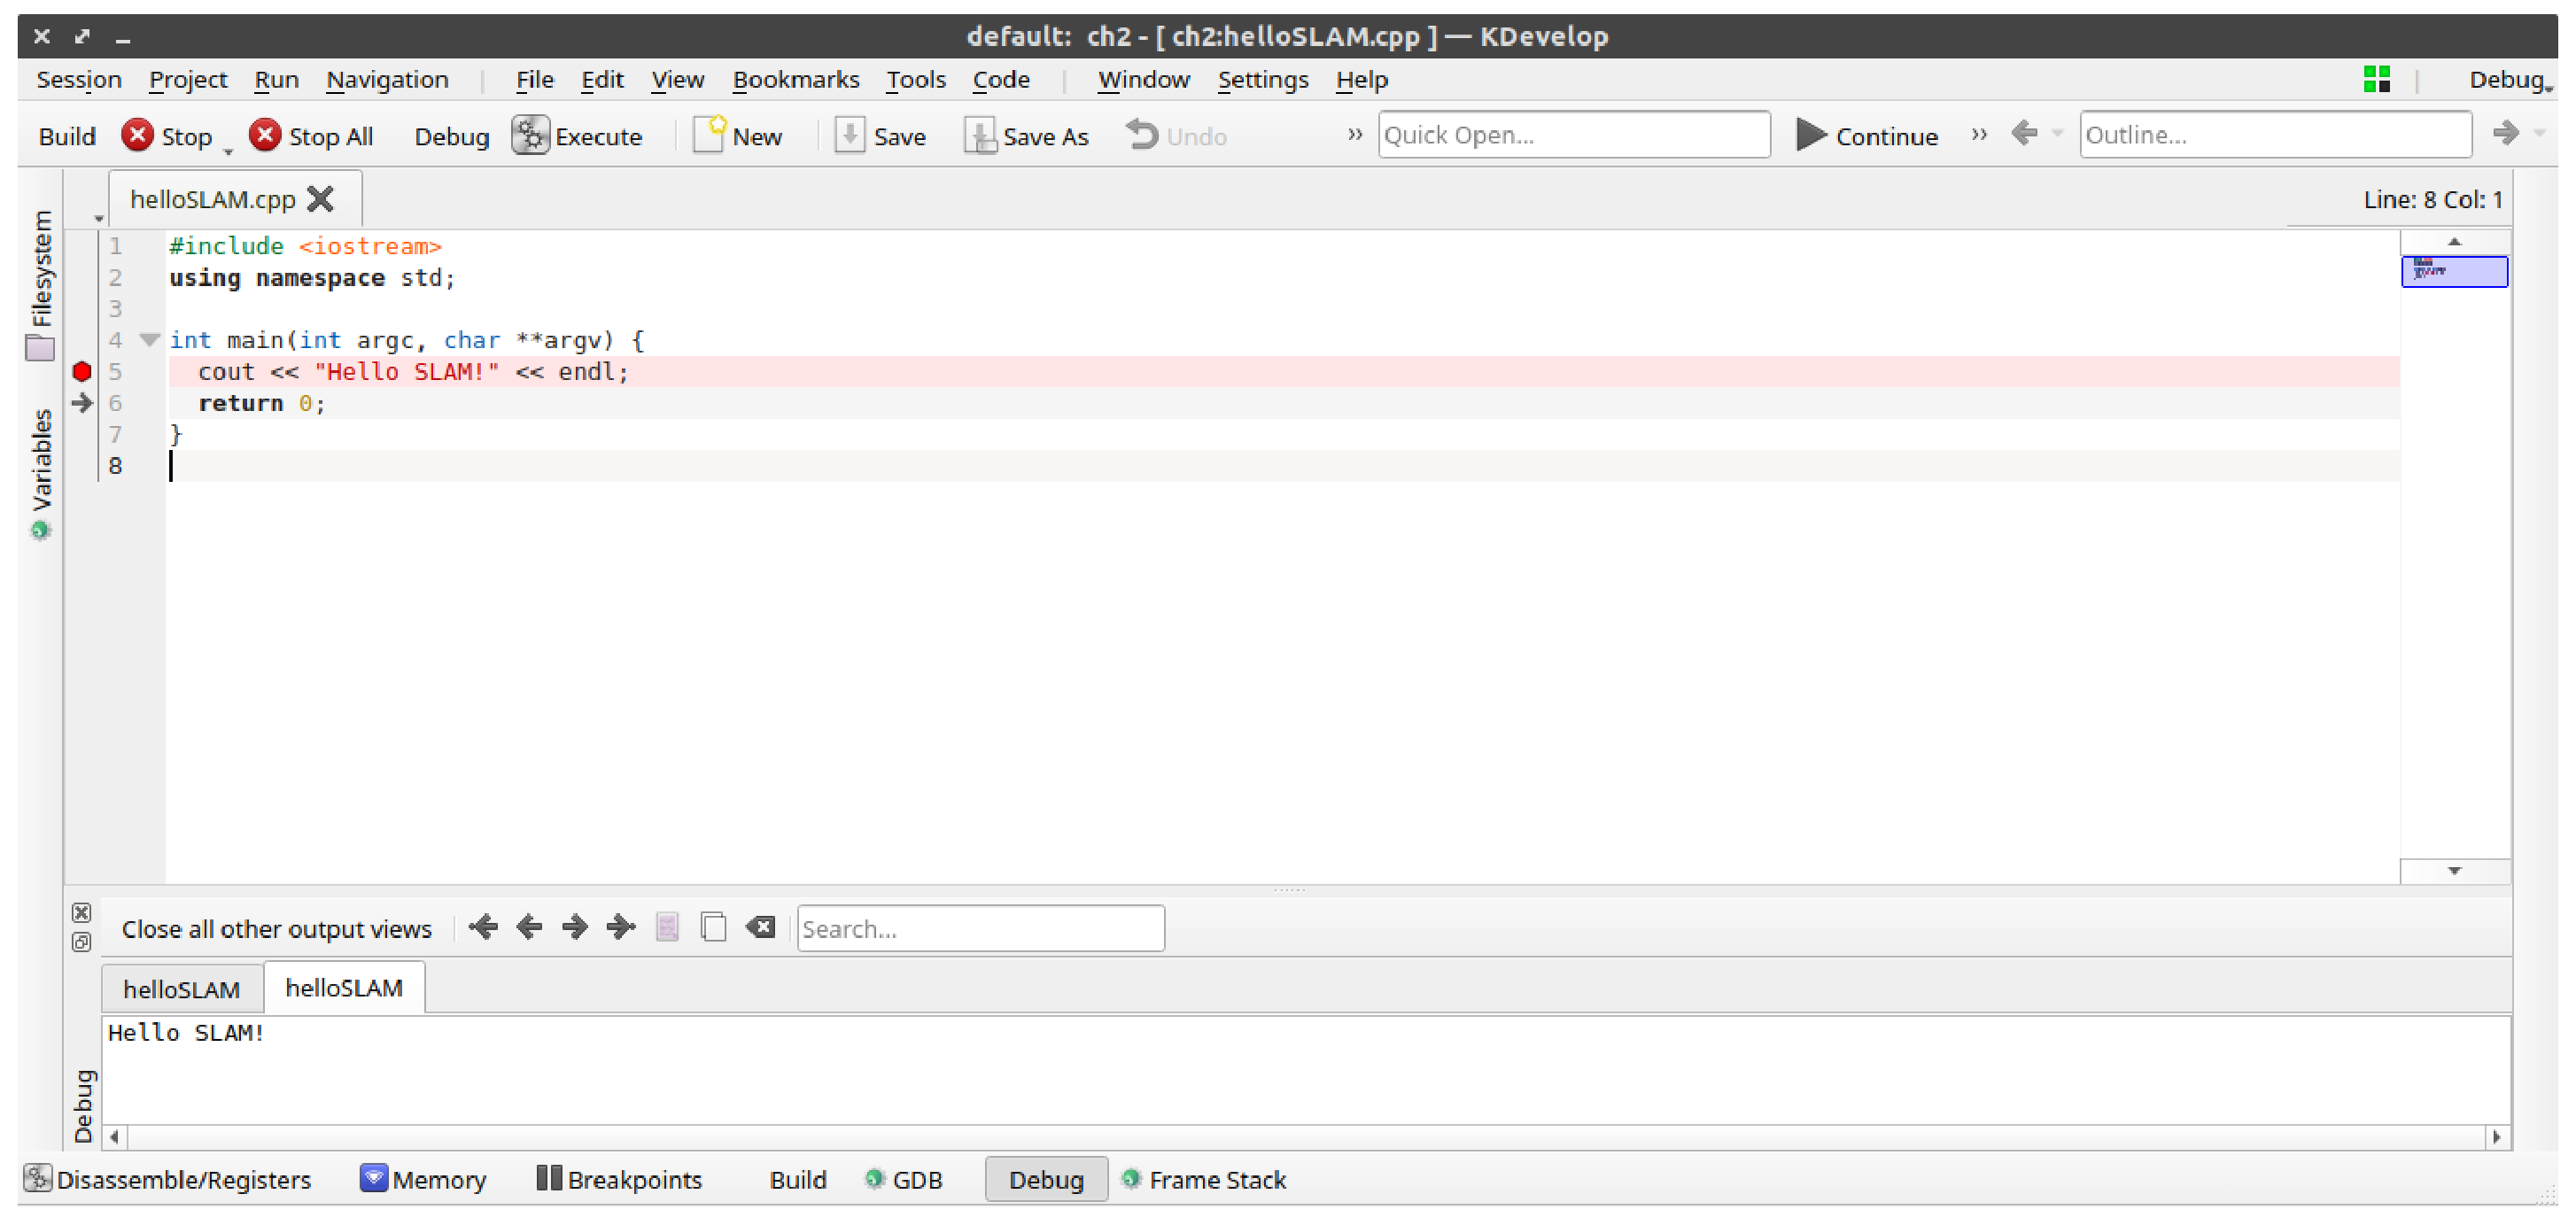
\includegraphics[width=0.8\textwidth]{whatIsSLAM/debug.pdf}
    \caption{Debug interface. }
    \label{fig:debug}
\end{figure}

When debugging, KDevelop will switch to debug mode and the interface will change a bit. At the breakpoint, you can control the operation of the program with single step operation (F10 key), single step follow up (F11 key), and single step jump (F12 key) function. At the same time, you can click the interface on the left to view the value of the local variable. Or select the ``Stop'' button to end debugging. After debugging, KDevelop will return to the normal development interface.

Now you should be familiar with the entire process of breakpoint debugging. In the future, if an error occurs during the running phase of the program, causing the program to crash, you can use breakpoint debugging to determine the location of the error, and then modify \footnote{ instead of directly sending us an email asking how to deal with the problem. }.

\subsubsection{Use Clion}
\begin{figure}[!t]
    \centering
    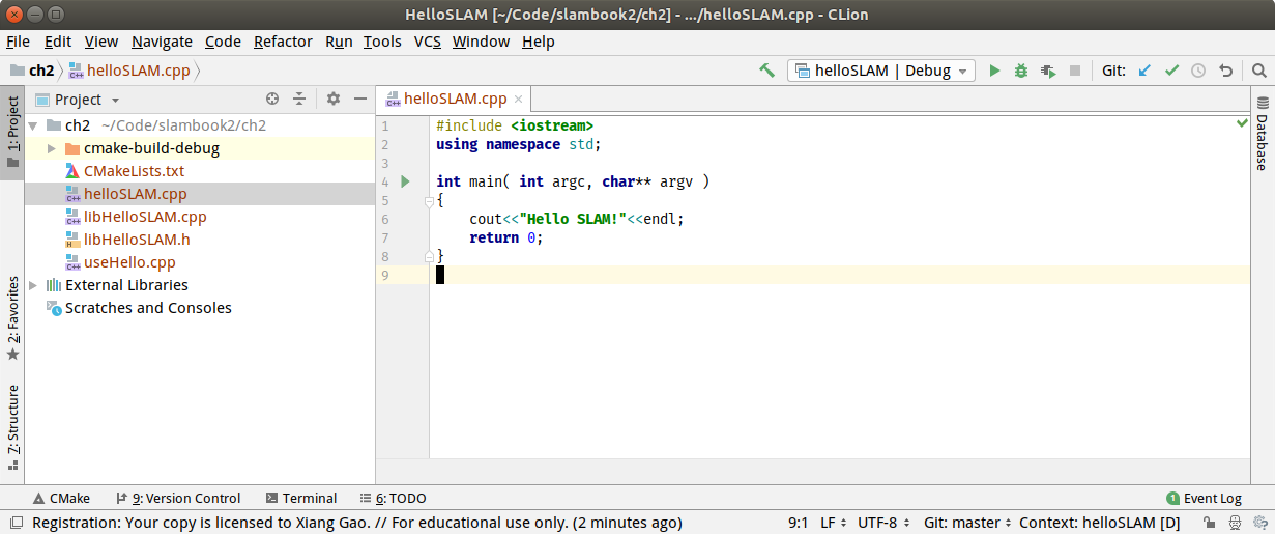
\includegraphics[width=1.0\textwidth]{whatIsSLAM/clion.pdf}
    \caption{Clion interface}
    \label{fig:clion}
\end{figure}

Clion is more complete than KDevelop, but it requires a user account, and the memory/CPU requirements for the host will be higher. \footnote{CLion is abnormally slow in the version after 2018. It is recommended that you use the release version around 2017. }. In Clion, you can also open a CMakeLists.txt or specify a directory. Clion will complete the cmake-make process for you. Its running interface is shown in \autoref{fig:clion}.

Similarly, after opening Clion, you can select the programs you want to run or debug in the upper right corner of the interface, and adjust their startup parameters and working directory. Click the small beetle button in this column to start the breakpoint debugging mode. Clion also has a number of convenient features, such as automatically creating classes, changing functions, and automatically adjusting the coding style. Please try it.

Ok, if you are already familiar with the use of the IDE, then the second chapter will stop here. You may already feel that I have talked too much, so in the following practice section, we will not introduce things like how to create a new build folder, call the cmake and make commands to compile the program. I believe that readers should master these simple steps. Similarly, since most of the third-party libraries used in this book are cmake projects, you will continue to be familiar with the compilation process. Next we will start the formal chapter and introduce some related mathematics.

\section*{Exercises}
\begin{enumerate}
    \item Read the survey SLAM literature~\cite{Liu2016} and~\cite{Liang2013}, can you read the contents? (They are Chinese papers for beginners. For English reader, see the next  exercise.)
    \item[\optional] Read SLAM's review literature, such as~\cite{Cadena2016, Fuentes-Pacheco2015, Boal2014, Chen2012, Chen2007} and so on. What are the similarities and differences between these papers on SLAM and this book?
    \item What are the parameters of the g++ command? If I want to change the generated program file name, how should I call g++?
    \item Use the build folder to compile your cmake project, then try it in KDevelop.
    \item Deliberately add some syntax errors to the code to see what information the build will generate. Can you read the error message of g++?
    \item If you forgot to link the library to the executable, will the compiler report an error? What kind of mistakes are reported?
    \item[\optional] Read ``cmake practice'' (or other cmake materials) to learn about the grammars of cmake.
    \item[\optional] Improve the hello SLAM problem, make it a small library, and install it on your local hard drive. Then, create a new project, use find\_package to find the library and call it.
    \item[\optional] Read other cmake instructional materials, such as \url{https://github.com/TheErk/CMake-tutorial}.
    \item Find the official website of KDevelop and see what other features it has. Are you using it?
    \item If you learned Vim in the last lecture, please try KDevelop's/Clion's Vim editing function.
\end{enumerate}